% Options for packages loaded elsewhere
\PassOptionsToPackage{unicode}{hyperref}
\PassOptionsToPackage{hyphens}{url}
\PassOptionsToPackage{dvipsnames,svgnames*,x11names*}{xcolor}
%
\documentclass[
]{article}
\usepackage{lmodern}
\usepackage{amssymb,amsmath}
\usepackage{ifxetex,ifluatex}
\ifnum 0\ifxetex 1\fi\ifluatex 1\fi=0 % if pdftex
  \usepackage[T1]{fontenc}
  \usepackage[utf8]{inputenc}
  \usepackage{textcomp} % provide euro and other symbols
\else % if luatex or xetex
  \usepackage{unicode-math}
  \defaultfontfeatures{Scale=MatchLowercase}
  \defaultfontfeatures[\rmfamily]{Ligatures=TeX,Scale=1}
\fi
% Use upquote if available, for straight quotes in verbatim environments
\IfFileExists{upquote.sty}{\usepackage{upquote}}{}
\IfFileExists{microtype.sty}{% use microtype if available
  \usepackage[]{microtype}
  \UseMicrotypeSet[protrusion]{basicmath} % disable protrusion for tt fonts
}{}
\makeatletter
\@ifundefined{KOMAClassName}{% if non-KOMA class
  \IfFileExists{parskip.sty}{%
    \usepackage{parskip}
  }{% else
    \setlength{\parindent}{0pt}
    \setlength{\parskip}{6pt plus 2pt minus 1pt}}
}{% if KOMA class
  \KOMAoptions{parskip=half}}
\makeatother
\usepackage{xcolor}
\IfFileExists{xurl.sty}{\usepackage{xurl}}{} % add URL line breaks if available
\IfFileExists{bookmark.sty}{\usepackage{bookmark}}{\usepackage{hyperref}}
\hypersetup{
  pdftitle={CoronaNet: A Dyadic Dataset of Government Responses to the COVID-19 Pandemic},
  pdfauthor={Cindy Cheng1,; Joan Barceló2; Allison Spencer Hartnett3; Robert Kubinec2; Luca Messerschmidt1},
  colorlinks=true,
  linkcolor=Maroon,
  filecolor=Maroon,
  citecolor=Blue,
  urlcolor=blue,
  pdfcreator={LaTeX via pandoc}}
\urlstyle{same} % disable monospaced font for URLs
\usepackage[margin=1in]{geometry}
\usepackage{longtable,booktabs}
% Correct order of tables after \paragraph or \subparagraph
\usepackage{etoolbox}
\makeatletter
\patchcmd\longtable{\par}{\if@noskipsec\mbox{}\fi\par}{}{}
\makeatother
% Allow footnotes in longtable head/foot
\IfFileExists{footnotehyper.sty}{\usepackage{footnotehyper}}{\usepackage{footnote}}
\makesavenoteenv{longtable}
\usepackage{graphicx}
\makeatletter
\def\maxwidth{\ifdim\Gin@nat@width>\linewidth\linewidth\else\Gin@nat@width\fi}
\def\maxheight{\ifdim\Gin@nat@height>\textheight\textheight\else\Gin@nat@height\fi}
\makeatother
% Scale images if necessary, so that they will not overflow the page
% margins by default, and it is still possible to overwrite the defaults
% using explicit options in \includegraphics[width, height, ...]{}
\setkeys{Gin}{width=\maxwidth,height=\maxheight,keepaspectratio}
% Set default figure placement to htbp
\makeatletter
\def\fps@figure{htbp}
\makeatother
\setlength{\emergencystretch}{3em} % prevent overfull lines
\providecommand{\tightlist}{%
  \setlength{\itemsep}{0pt}\setlength{\parskip}{0pt}}
\setcounter{secnumdepth}{5}
\linespread{1.6}
\usepackage{lineno}
\linenumbers
\usepackage{booktabs}
\usepackage{longtable}
\usepackage{array}
\usepackage{multirow}
\usepackage{wrapfig}
\usepackage{float}
\usepackage{colortbl}
\usepackage{pdflscape}
\usepackage{tabu}
\usepackage{threeparttable}
\usepackage{threeparttablex}
\usepackage[normalem]{ulem}
\usepackage{makecell}
\usepackage{xcolor}
\newlength{\cslhangindent}
\setlength{\cslhangindent}{1.5em}
\newenvironment{cslreferences}%
  {}%
  {\par}

\title{CoronaNet: A Dyadic Dataset of Government Responses to the COVID-19 Pandemic}
\author{Cindy Cheng\textsuperscript{1,*} \and Joan Barceló\textsuperscript{2} \and Allison Spencer Hartnett\textsuperscript{3} \and Robert Kubinec\textsuperscript{2} \and Luca Messerschmidt\textsuperscript{1}}
\date{April 24th, 2020}

\begin{document}
\maketitle
\begin{abstract}
Governments everywhere have implemented numerous policies that have been influential in shaping the COVID-19 pandemic. We present an initial public release of a large hand-coded dataset of over 12,000 separate policy announcements in response to the pandemic across more than 190 countries. The dataset is updated daily, with a 5-day lag for validity checking. We document policies across numerous dimensions, including the type of policy; national vs.~sub-national enforcement; the specific human group and geographic region targeted by the policy; and the time frame within which the policy is implemented. We further analyze the dataset using a Bayesian measurement model which shows the quick acceleration of the adoption of costly policies across countries beginning in mid-March and continuing to the present. Furthermore, we find that the rate of policy adoption varied widely across countries, with New Zealand having the fastest response across policy categories and the United States the most gradual.
\end{abstract}

\textsuperscript{1} Hochschule für Politik at the Technical University of Munich (TUM) and the TUM School of Governance, Munich, Germany\\
\textsuperscript{2} Social Science Division, New York University Abu Dhabi, Abu Dhabi, UAE\\
\textsuperscript{3} Department of Political Science, Yale University, New Haven, USA

\textsuperscript{*} Correspondence: \href{mailto:cindy.cheng@hfp.tum.de}{Cindy Cheng \textless{}\href{mailto:cindy.cheng@hfp.tum.de}{\nolinkurl{cindy.cheng@hfp.tum.de}}\textgreater{}}

\newpage

Governments all around the world have implemented an astonishing number and variety of policies in reaction to the COVID-19 pandemic in a very short time frame. However, policy makers and researchers have to date lacked access to the quality, up-to-date data they need for conducting rigorous analyses of whether, how, and to what degree these fast changing policies have worked in brunting the health, political and economic effects of the pandemic. To address this concern, in this paper, we present the CoronaNet COVID-19 Government Response Database, which provides fine-grained, dyadic data on policy actions taken by governments across the world since the Chinese government reported the COVID-19 outbreak on December 31, 2019. At the time of writing, the dataset covers the policy actions of 194 countries\footnote{Note, we will include additional countries in future versions of the dataset.} up until 2020-04-29, for a total of 13074 events.

With the help of a team of over 260 research assistants in 18 time zones, we are releasing the data on a daily basis. We are implementing a five-day lag between data collection and release to evaluate and validate ongoing coding efforts for random samples of the data to ensure the best possible quality given the considerable time constraints. More specifically, the CoronaNet database collects daily data on government policy actions taken against COVID-19 across the following dimensions:

\begin{itemize}
\tightlist
\item
  The type of government policy implemented (e.g.~quarantine, closure of schools {[}16 total{]})
\item
  The level of government initiating the action (e.g.~national, provincial)
\item
  The geographical target of the policy action, if applicable (e.g.~national, provincial, municipal)
\item
  The human or material target of the policy action, if applicable (e.g.~travelers, masks)
\item
  The directionality of the policy action, if applicable (e.g.~inbound, outbound, both)
\item
  The mechanism of travel that the policy action targets, if applicable (e.g.~flights, trains)
\item
  The compliance with the policy action (e.g.~mandatory, voluntary)
\item
  The enforcer of the policy action (e.g.~national government, military)
\item
  The timing of the policy action (e.g.~date announced, date implemented)
\end{itemize}

Though government responses to the COVID-19 pandemic have inaugurated unprecedented changes in how billions of people live their lives, they draw on the lessons learned from the endless series of pandemics and epidemics that came before. Indeed, the earliest written sources document how ancient Mesopotamian responded to the constant threat of epidemic by, on the one hand appealing to various ``healing goddesses'\,' and on the other hand, isolating people showing the first symptoms of a disease from others.\textsuperscript{1,2} As time has marched forward, pandemics and epidemics have consistently and dramatically changed the course of human history\textsuperscript{3--7} and governments have continued to implement a variety of policies in response.\textsuperscript{1,8,9}\footnote{Note that early historical guidelines for responding to epidemics can also be found in a number of early texts, e.g.~the Bible contains a number of references to the use of quarantine to address the problem of leprosy including Leviticus 13:46 ``As long as they have the disease they remain unclean. They must live alone; they must live outside the camp.''} Throughout this all, the collection of and access to reliable data, has helped advance collective understanding of which policies are actually effective in curbing the effects of a given pandemic.\textsuperscript{10,11} This is no trivial task given that a policy that is effective in one context may be ineffective in another due to a whole host of potentially conditioning factors, including the pathogenesis of the particular disease,\textsuperscript{12,13} the characteristics of the underlying population,\textsuperscript{14--17} and the available medical\textsuperscript{18,19} and communication\textsuperscript{20--23} technology at the time.

We believe that the data presented in this paper will be similarly invaluable for helping policy makers and researchers assess how effective different policies are in addressing the spread and health outcomes of COVID-19.\textsuperscript{24} While available research is necessarily preliminary, it suggests that which policies governments have implemented in response to COVID-19,\textsuperscript{25--27} when they decided to implement them,\textsuperscript{29,30} who they were targeted toward\textsuperscript{31,32} and what state capacity they possessed to do so\textsuperscript{33,34} have all significantly influenced how the virus has affected health outcomes both within and across different country contexts,\textsuperscript{35,36} and which is readily captured by our dataset. Equally important is understanding why countries adopt different policies, with early analyses suggesting that institutional and political factors, e.g.~the authoritarian or democratic nature of a country's institutions\textsuperscript{37} or its level of political partisanship,\textsuperscript{38} play an important role. These findings will not only improve the global response to the current crisis, but can also build an influential foundation of knowledge for responding to future outbreaks.\textsuperscript{39,40}

Meanwhile, given the exogenous timing of the initial outbreak in Wuhan, China, government policies made in reaction to the COVID-19 pandemic constitute the single largest natural experiment in recent memory, allowing researchers to improve causal inference in any number of fields. Indeed, government reactions to the COVID-19 epidemic may forward our understanding of a wide-range of social phenomena, from the evolution of political institutions\textsuperscript{41--45} to the progression of economic development\textsuperscript{46--50} and the stability of financial markets\textsuperscript{51,52} to say nothing of what we might learn about what we might learn about environmental economics,\textsuperscript{53,54} mental health,\textsuperscript{55,56} disaster response\textsuperscript{57,58} and disaster preparedness.\textsuperscript{59--61} Some initial analyses suggest that the COVID-19 pandemic has already led to authoritarian backsliding in some countries,\textsuperscript{62} unprecedented shocks to the economy,\textsuperscript{63,64} and serious negative mental health effects for millions of people.\textsuperscript{65,66} While scholars have always sought to understand how large-scale historical events have shaped contemporary phenomena, modern technological tools allow us to document such events more quickly and more precisely than ever before.

In what follows, we provide a description of the data, as well as an application of the data in which we model policy activity of countries over time. Using a Bayesian dynamic item-response theory model, we produce a statistically valid index that summarizes countries in terms of their response to the pandemic, and further shows how quickly policy responses have changed over time. We document clear evidence of rapid policy diffusion of harsh measures opposing the virus, indicating some of the most extensive evidence of this type of diffusion ever documented. In the methodology section, we provide a thorough discussion of the procedures used to collate the data and to manage the more than 260 research assistants coding this data around the world in real time.

\hypertarget{results}{%
\section*{Results}\label{results}}
\addcontentsline{toc}{section}{Results}

In this section, we first present some descriptive statistics that illustrate how government policy toward COVID-19 has varied across key variables. We then briefly present our new index for tracking how active governments have been with regard to announcing policies targeting COVID-19 across countries and over time.

\hypertarget{descriptive-statistics}{%
\subsection*{Descriptive Statistics}\label{descriptive-statistics}}
\addcontentsline{toc}{subsection}{Descriptive Statistics}

Here we present some descriptive statistics for key variables available in the data. Table \ref{tab:desctab} shows the number of records for each policy type (please see Data Schema section for more information on how a policy type is defined), the number of unique countries for each policy type, how many countries are targeted in total by each policy type and the degree to which a given policy must be complied with. We present cumulative totals for the different categories in the data, except for the number of targeted countries, which is an average number. While, we highlight the number of targeted countries in this table, we note that our data also captures other potential geographic targets. For instance, it is possible for a national policy to be targetd toward a particular sub-national province or a provincial policy to be targeted toward a certain sub-provincial regions.

Table \ref{tab:desctab} shows that the most common government policy implemented in reaction to COVID-19 is external border restrictions, i.e.~policies that seek to limit access to ports of entry or exit across different governmental jurisdictions. We find that 182 countries have made 1850 policy announcements about such restrictions since December 31, 2019. Meanwhile, the second policy that most countries, by our count 162, have implemented is `Closure of Schools', of which we document 1573 such policies. Governments have implemented `Restriction of Non-Essential Businesses' policies with the second highest frequency; we document that 132 countries have implemented 1787 such policies. However, we note that a strict comparison of policy types by this metric is not perfect, given that, for example, there may be a need for more individualized policies regarding external border restrictions (given the number of countries which a government can restrict travel access to) as opposed to closing schools. In the next subsection, we provide a more rigorous method of comparing policies while taking their depth into account.

Meanwhile, our dataset also shows that virtually all countries in the world are a target of an external border restriction, quarantine measure, or health monitoring measure from another country. Moreover, a high percentage of policies documented in our dataset have mandatory enforcement.

\begin{table}[H]

\caption{\label{tab:desctab}Descriptive Information about the CoronaNet Government Response Dataset}
\centering
\begin{tabular}[t]{>{\raggedright\arraybackslash}p{4cm}>{\raggedleft\arraybackslash}p{2.5cm}>{\raggedleft\arraybackslash}p{2.5cm}>{\raggedleft\arraybackslash}p{2.5cm}>{\raggedleft\arraybackslash}p{2.5cm}}
\toprule
Type & Total Number of Policies & Number of Countries & Average Number of Targeted Countries & \% With Mandatory Enforcement\\
\midrule
\rowcolor{gray!6}  Health Resources & 2247 & 140 & 148 & 59\\
External Border Restrictions & 1850 & 182 & 205 & 79\\
\rowcolor{gray!6}  Restriction of Non-Essential Businesses & 1787 & 132 & 133 & 92\\
Closure of Schools & 1573 & 162 & 162 & 88\\
\rowcolor{gray!6}  Quarantine/Lockdown & 1135 & 153 & 206 & 88\\
\addlinespace
Other & 872 & 127 & 143 & 60\\
\rowcolor{gray!6}  Restrictions of Mass Gatherings & 669 & 153 & 154 & 87\\
Public Awareness Measures & 604 & 130 & 131 & 26\\
\rowcolor{gray!6}  Social Distancing & 508 & 119 & 119 & 69\\
Declaration of Emergency & 489 & 113 & 114 & 100\\
\addlinespace
\rowcolor{gray!6}  Restriction of Non-Essential Government Services & 373 & 91 & 91 & 87\\
Health Monitoring & 365 & 110 & 202 & 74\\
\rowcolor{gray!6}  Internal Border Restrictions & 356 & 109 & 109 & 89\\
New Task Force, Bureau or Administrative Configuration & 318 & 95 & 95 & 56\\
\rowcolor{gray!6}  Health Testing & 280 & 89 & 112 & 65\\
\addlinespace
Curfew & 215 & 91 & 89 & 97\\
\rowcolor{gray!6}  Hygiene & 23 & 9 & 9 & 96\\
Anti-Disinformation Measures & 2 & 2 & 2 & 100\\
\bottomrule
\end{tabular}
\end{table}

In addition, we can look at the cumulative incidence of different types of policies in our data over time, as we show in Figure \ref{fig:overtime}. The figure shows that relatively easy to implement policies like external border restrictions, the forming of task forces, public awareness campaigns, and efforts to increase health resources came relatively earl in the course of the pandemic. More restrictive policies like curfews, closures of schools, restrictions of non-essential businesses and restrictions of mass gatherings arrived later.

\begin{figure}
\centering
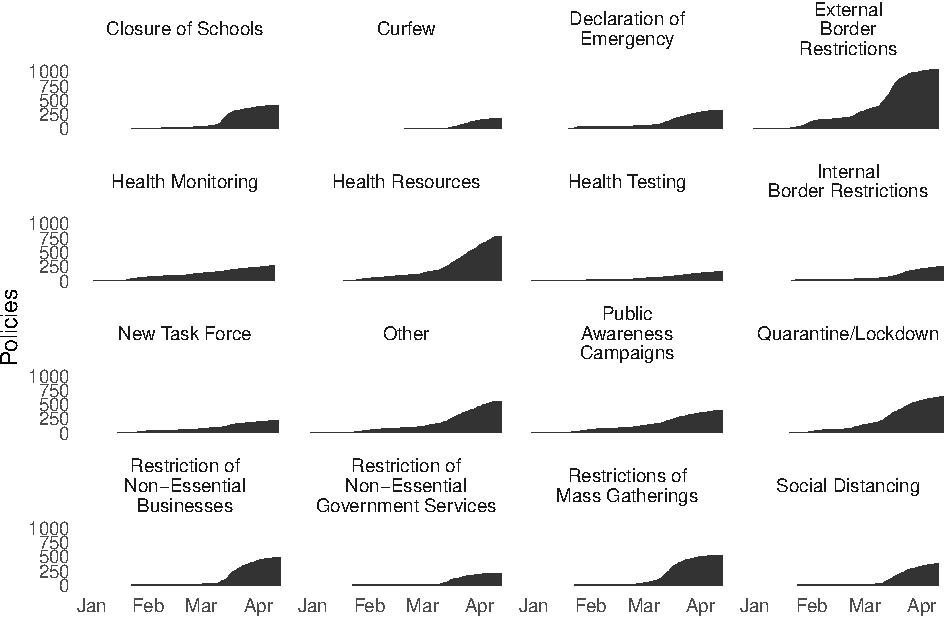
\includegraphics{corona_wp_R1_nature_files/figure-latex/overtime-1.pdf}
\caption{\label{fig:overtime}Cumulative Incidence of Policy Event Types Over Time}
\end{figure}

We can also explore the extent to which other countries are affected by policies that can have a geographic target outside the policy initiator (e.g.~`external border restrictions', `quarantine') across time. For example, in Figure \ref{fig:biofe}, we map a network of bans on inbound flights to European countries initiated by European countries\footnote{In this paper, the following countries are defined as being in Europe: Albania, Andorra, Armenia, Austria, Belarus, Belgium, Bosnia and Herzegovina, Bulgaria, Croatia, Cyprus, Czech Republic, Denmark, Estonia, Finland, France, Georgia, Germany, Greece, Hungary, Iceland, Ireland, Italy, Kosovo, Latvia, Liechtenstein, Lithuania, Luxembourg, Macedonia, Malta, Moldova, Monaco, Montenegro, Netherlands, Norway, Poland, Portugal, Romania, San Marino, Serbia, Slovakia, Slovenia, Spain, Sweden, Switzerland, Ukraine, United Kingdom, and the Vatican.} as of March 15, 2020. In the plot, each horizontal line represents a potential geographical target of a flight ban. The vertical lines denote whether there was such a flight ban and the arrow of the vertical line indicates the direction in which the ban is applied.\footnote{See 67 for more information on how to interpret this plot.} The figure shows that by March 15, 2020, the governments of Poland and San Marino had banned all flights into Poland and San Marino respectively while the government of Italy banned incoming flights from China, Hong Kong, Macau and Taiwan. Additionally, the governments of Greece and Romania both banned flights from Italy while the government of Albania banned incoming flights from Greece. According to our data, up until this point in time, no other European governments at the national level had banned inbound flights from other countries.\footnote{However, at the provincial level, our dataset documents that the government of the autonomous region of Madeira, Portugal had banned flights from Denmark, Finland, France, Germany, Spain, and Switzerland while the government of Sardinia, Italy closed all airports by March 15, 2020.}

\begin{figure}
\centering
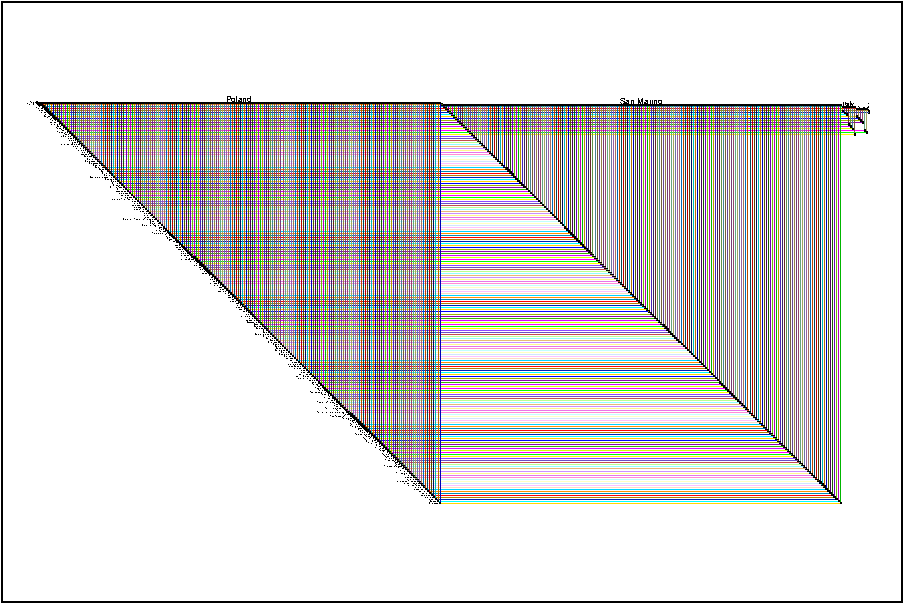
\includegraphics{corona_wp_R1_nature_files/figure-latex/biofe-1.pdf}
\caption{\label{fig:biofe}Network Map of Bans on Inbound Flights by European Countries as of March 15, 2020}
\end{figure}

\hypertarget{government-policy-activity-index}{%
\section*{Government Policy Activity Index}\label{government-policy-activity-index}}
\addcontentsline{toc}{section}{Government Policy Activity Index}

In this section, we briefly present our new index for tracking the relative government activity with regards to policies targeting COVID-19 across countries and over time. The model is a version of item-response theory known as ideal point modeling that incorporates over-time trends,\textsuperscript{68--73} permitting inference on how a latent construct, in this case total policy activity, responds to changes in the pandemic. To fit the model, the different policy types shown in Table \ref{tab:desctab} were coded in terms of ordinal values, with lower values for sub-national targets of policies and higher values for policies applying to the entire country, or in the case of external border restrictions, to one or more external countries. For instance, internal country policies can take on three possible values: no policy, sub-national policy, or policy covering the whole country. Meanwhile external border restrictions can take on four possible values: no policy, policy targeting one other country, policy targeting multiple countries, and policy targeting all countries in the world (i.e., border closure).

We employed ideal point modeling because it can be given a latent utility interpretation.\textsuperscript{69} We assume that each country has an unobserved ``ideal point'' on a unidimensional space representing its willingness to impose policies, while each policy likewise has a position on the same space. The relative cost of different policies can be thought of as the distance between a country's ideal point and the ideal point of the policy relative to other policies. While the meaning of this implied cost will vary from country to country, it is likely a combination of the social, political and economic costs of implementing the policy at a given time point.

As countries become more willing to pay the implied cost (i.e.~the latent distance between country and policy decreases), the country's ideal points/policy activity score will rise and they will implement more policies. This interpretation is similar to the traditional item-response theory approach for analyzing test questions in which students who correctly answer more questions on a test are considered to have higher ``ability''.\textsuperscript{74,75} Following this logic, we are able to estimate latent country scores that represent the readiness of a country to impose a set number of policies. The implied cost of policies is estimated via discrimination parameters, which indicate how strongly policies discriminate between countries.

The country-level policy activity score is further allowed to vary over time in a random-walk process with a country-specific variance parameter to incorporate heteroskedasticity.\textsuperscript{71} Incorporating over-time trends explicitly is very important for capturing the nuances of policy implementation over time. For example, countries that impose more restrictive policies at an earlier date will be rewarded with higher policy activity scores compared to those who impose such policies at a later date. Imposing a given policy when most countries have already imposed them will result in little if any change in the policy activity score.

The advantage of employing a statistical model, rather than simply summing across policies, is that the index ends up as a weighted average, where the weights are derived from the probability that a certain policy is implemented. In other words, while many countries set up task forces, relatively few imposed curfews at an early stage. As a result, the model adjusts for these distinctions, producing a score that aggregates across the patterns in the data.

Furthermore, because the model is stochastic, it is robust to some of the coding errors of the kind that often occur in these types of datasets. As we discuss in our validation section, while we are continuing to validate the data on a daily basis, the massive speed and scope of data collection means that we cannot identify all issues with the data in real time. However, the measurement model employed only requires us to assume that on average the policy codings are correct, not that they are correct for each instance. Coding error, such as incorrectly selecting a policy type, will propagate through the model as higher uncertainty intervals, but will not affect average posterior estimates. As our data quality improves, and we are able to collect more data over time, the model will produce more variegated estimates with smaller uncertainty intervals.

Figure \ref{fig:plotindex} shows the estimated index scores for the 194 countries in our dataset at present, and suggests strong evidence of policy diffusion effects. While information about COVID-19 existed at least as early as January, we do not see large-scale changes occurring in activity scores until March. Furthermore, the trajectories are highly non-linear, with a large number of countries quickly transitioning from relatively low to relatively high scores. This non-linear movement could be due to a variety of factors, including the rapid spread of the virus and policy learning as states observe other states' policy actions. We note that the country that appeared to take the quickest action in the shortest amount of time is New Zealand, as can be seen in Figure \ref{fig:plotvar} where we show over-time variance parameters for each country.

Of course, a caveat with the index is that we may be missing some possible policy measures that have occurred due to the difficulty in finding them in published sources. However, there is still clear differentiation within the index in terms of when policies were imposed, with some countries starting to impose policies much earlier than others. Furthermore, there is a clear break about March 1st when countries began to impose more stringent policies across the world.

\begin{figure}
\centering
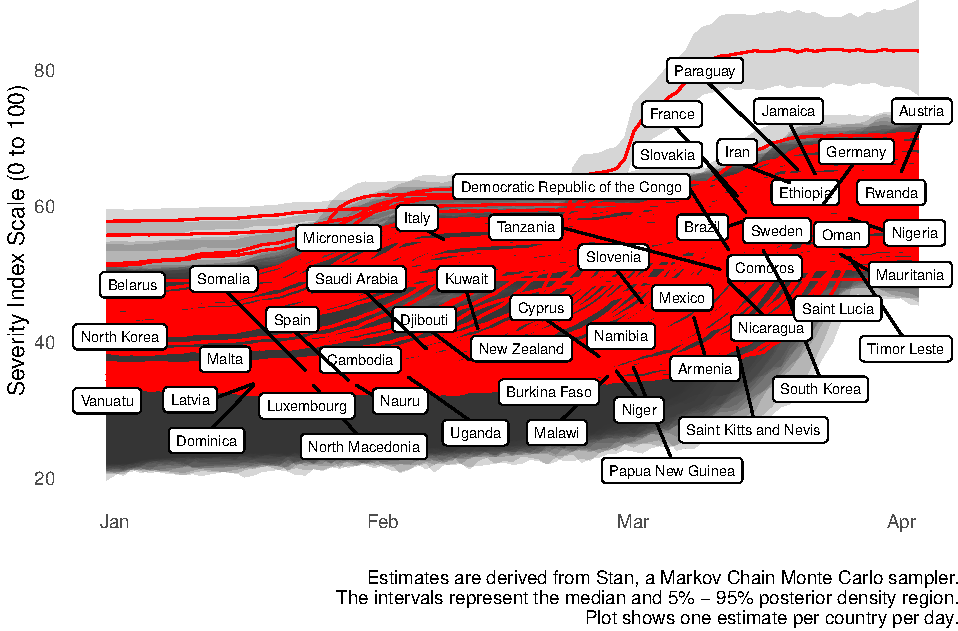
\includegraphics{corona_wp_R1_nature_files/figure-latex/plotindex-1.pdf}
\caption{\label{fig:plotindex}CoronaNet Time-Varying Index of National Policy Activity of Measures Opposing COVID-19 Pandemic}
\end{figure}

Table \ref{tab:rankcount} shows the discrimination parameters from the underlying Bayesian model for each policy type. These parameters suggest which policies governments find relatively difficult or costly to implement, and for that reason tend to separate more active from less active states in terms of response to COVID-19. Two of these policies (Closure of Restaurants and Quarantine at Home) were given fixed values in order to identify the direction and rotation of the latent scale, and so their discrimination parameters are not informative. These policies were chosen as a priori we can identify them as being relatively high cost. However, the rest of the parameters were allowed to float, which provides inference as to which policies appear to be the most difficult/costly to implement.

We note that these are average values for the sample. Imposing these policies may be less costly for certain countries or for countries that share certain characteristics, such as having smaller numbers of enrolled students or relatively healthy economies. However, it is important to note that we can see these patterns on a world-wide scale.

At the top of the index we see various business closure policies as the most difficult to implement, while school closures are the next most difficult. Closure of pre-schools, though, as opposed to other school types, appears to be relatively less costly for states to undertake, perhaps because pre-schools do not operate on a full-time basis. Internal border restrictions are considered more difficult to implement than external border restrictions, while relatively straightforward policies like public awareness campaigns, health monitoring and opening new task forces or bureaus are near the bottom of the index. Quarantines placing people in external facilities, such as hotels or government quarantine centers, are also estimated as being less costly than quarantine at home (stay-at-home orders).

Given this distribution of discrimination parameters, we believe the index is a valid representation of the underlying process by which governments progressively impose more difficult policies. As states relax policies, we will further gain information about which policies appear to be more costly as we will be able to factor in the duration for which these policies were implemented. Consistent with our findings, we observe that the announced relaxation policies happening at the time of writing in European countries primarily center on businesses and school openings, suggesting that these policies are uniquely costly to keep in place compared to travel restrictions.\footnote{See Doherty, Ben. ``The exit strategy: how countries around the world are preparing for life after Covid-19.'' \emph{The Guardian} 18 April 2020, \url{https://www.theguardian.com/world/2020/apr/19/the-exit-strategy-how-countries-around-the-world-are-preparing-for-life-after-covid-19}}

\begingroup\fontsize{9}{11}\selectfont

\begin{longtable}[t]{>{\raggedright\arraybackslash}p{4cm}>{\raggedleft\arraybackslash}p{2.5cm}>{\raggedleft\arraybackslash}p{2.5cm}>{\raggedleft\arraybackslash}p{2.5cm}>{}p{2.5cm}}
\caption{\label{tab:rankcount}Discrimination of Item Parameters (Policies) in Policy Activity Index}\\
\toprule
Policy & 5\% Low Estimate & Median Estimate & 95\% High Estimate\\
\midrule
\rowcolor{gray!6}  Closure of Shopping Malls & 1.5 & 1.7 & 2.0\\
Restriction Commercial Business & 1.5 & 1.7 & 1.9\\
\rowcolor{gray!6}  Closure of Retail Stores & 1.3 & 1.5 & 1.8\\
Closure of Personal Grooming & 1.2 & 1.4 & 1.6\\
\rowcolor{gray!6}  Primary School Closure & 1.1 & 1.3 & 1.4\\
\addlinespace
High School Closure & 1.1 & 1.2 & 1.4\\
\rowcolor{gray!6}  Higher Ed Closure & 1.0 & 1.1 & 1.2\\
Restriction Other Business & 0.9 & 1.1 & 1.2\\
\rowcolor{gray!6}  Sanitizer Policies & 0.9 & 1.0 & 1.2\\
Closure of Restaurants & 1.0 & 1.0 & 1.0\\
\addlinespace
\rowcolor{gray!6}  Quarantine At Home & 1.0 & 1.0 & 1.0\\
Pre-school Closure & 0.9 & 1.0 & 1.1\\
\rowcolor{gray!6}  Mobilization of Volunteers & 0.8 & 0.9 & 1.1\\
Other Health Staff & 0.8 & 0.9 & 1.0\\
\rowcolor{gray!6}  Restriction of Mass Gatherings & 0.8 & 0.9 & 1.0\\
\addlinespace
Test Production & 0.7 & 0.8 & 1.0\\
\rowcolor{gray!6}  Mobilization of Doctors & 0.7 & 0.8 & 1.0\\
Mobilization of Nurses & 0.7 & 0.8 & 1.0\\
\rowcolor{gray!6}  Internal Border Restrictions & 0.7 & 0.8 & 0.9\\
Limited Quarantine & 0.6 & 0.8 & 1.0\\
\addlinespace
\rowcolor{gray!6}  Other Health Resources & 0.7 & 0.8 & 0.9\\
Social Distancing & 0.7 & 0.8 & 0.9\\
\rowcolor{gray!6}  Other Health Facilities & 0.6 & 0.8 & 0.9\\
Other Health Resources & 0.6 & 0.8 & 0.9\\
\rowcolor{gray!6}  Mobilization of Ventilators & 0.6 & 0.8 & 0.9\\
\addlinespace
Masks Policies & 0.6 & 0.7 & 0.9\\
\rowcolor{gray!6}  Restriction Government Services & 0.6 & 0.7 & 0.8\\
Other Health Facilities & 0.5 & 0.7 & 0.8\\
\rowcolor{gray!6}  PPE Mobilization & 0.5 & 0.6 & 0.8\\
External Border Closure & 0.6 & 0.6 & 0.7\\
\addlinespace
\rowcolor{gray!6}  Supporting Hospitals & 0.5 & 0.6 & 0.7\\
Other Quarantine & 0.5 & 0.6 & 0.7\\
\rowcolor{gray!6}  Quarantine in Hotel & 0.5 & 0.6 & 0.7\\
Curfew & 0.5 & 0.5 & 0.6\\
\rowcolor{gray!6}  Biomedical Research & 0.4 & 0.5 & 0.7\\
\addlinespace
Declaration of Emergency & 0.4 & 0.5 & 0.6\\
\rowcolor{gray!6}  Temporary Medical Units & 0.3 & 0.5 & 0.6\\
Quarantine/Lockdown & 0.3 & 0.4 & 0.6\\
\rowcolor{gray!6}  Building Quarantine Facilities & 0.3 & 0.4 & 0.5\\
Public Testing Mobilization & 0.3 & 0.4 & 0.5\\
\addlinespace
\rowcolor{gray!6}  Quarantine in Govt. Facility & 0.3 & 0.4 & 0.5\\
Border Health Certificates & 0.3 & 0.4 & 0.5\\
\rowcolor{gray!6}  Monitoring Population Health & 0.3 & 0.4 & 0.4\\
Public Awareness Measures & 0.3 & 0.3 & 0.4\\
\rowcolor{gray!6}  Suspend Visa Issuance & 0.3 & 0.3 & 0.4\\
\addlinespace
Mobilization of Testing & 0.3 & 0.3 & 0.4\\
\rowcolor{gray!6}  Task Force & 0.2 & 0.3 & 0.4\\
Other Border Restriction & 0.0 & 0.2 & 0.5\\
\rowcolor{gray!6}  Border Health Screenings & 0.2 & 0.2 & 0.3\\
Travel History Required & 0.1 & 0.1 & 0.2\\
\bottomrule
\end{longtable}
\endgroup{}

\hypertarget{methods}{%
\section*{Methods}\label{methods}}
\addcontentsline{toc}{section}{Methods}

In this section, we first describe the variables that our dataset provides as well as how they are organized. We then provide detail on the methodology we employed to collect the data.

\hypertarget{time-varying-item-response-model}{%
\subsection*{Time-Varying Item Response Model}\label{time-varying-item-response-model}}
\addcontentsline{toc}{subsection}{Time-Varying Item Response Model}

Our time-varying item response model follows the specification in 76. We review that notation here to show how it relates to classical item-response theory as well as the ideal point modeling literature.

The likelihood function for the model is as follows for a set of countries \(i \in I\), items \(j \in J\), time points \(t \in T\) and ordinal categories \(k \in K\):

\begin{align}
    L(Y_{ijtk}|\alpha_{it},\gamma_j,\beta_j) =  \prod_{i=1}^{I} \prod_{j=1}^{J} \prod_{t=1}^{T}
    \begin{cases} 
    1 -  \zeta(\gamma_j \alpha_{it} - \beta_j - c_1) & \text{if } K = 0 \\
    \zeta(\gamma_j \alpha_i - \beta_j - c_{k-1}) - \zeta(\gamma_j \alpha_{it} - \beta_j - c_{k})       & \text{if } 0 < k < K, \text{ and} \\
    \zeta(\gamma_j \alpha_{it} - \beta_j - c_{k-1}) - 0 & \text{if } k=K
    \end{cases}
\label{eq:basic}
\end{align}

In this equation, the time-varying country parameters \(\alpha_{it}\), also called person abilities or ideal points, are our estimate of policy activity scores. They are estimated jointly with the item (policy type) discrimination parameters \(\gamma_j\) and item difficulty (intercept) parameters \(\beta_j\). To address the ordinal nature of the outcome \(Y_{ijtk}\), ordinal cutpoints \(c_{k}\) are used to model the varying levels of enforcement and geographical targets in the data. The logit function, represented by \(\zeta(\cdot)\), maps the latent scale to probability that a given ordinal outcome is chosen. Because we have two separate type of ordered measures (domestic versus international policies) with either three or four ordered categories, we estimate the model jointly as two ordered logit specifications.

The likelihood in \eqref{eq:basic} is not fully identified due to possible scaling issues with the latent variable \(\alpha_{it}\) (i.e., it has no natural units) and due to potential sign reflection (also called multi-modality) where \(L(Y_{ijtk})\) could be unchanged even if \(\alpha_{it}\) is multiplied by -1. These identification issues are well-known in the literature,\textsuperscript{70} and we resolve them with standard practices. First, we assign a reasonably informative prior distribution on the \(t=1\) ideal points:

\begin{equation}
\alpha_{it=1} \sim N(0,1)
\label{eq:id1}
\end{equation}

We also fix the discrimination parameters \(\gamma_j\) for two items, quarantines and restriction of restaurants and bars, to opposite ends of the latent scale (+1 and -1). Because both of these variables load on the same side of the scale (i.e.~both indicate more policy activity), we reverse the order of the categories for restriction of restaurants and bars. We note that these types of restrictions are not commonly used in traditional IRT, where instead a sign restriction is imposed on all discrimination parameters. We employ the more flexible ideal point specification, which also allows us to test the assumption that all the discrimination parameters load on the same sign (as Table \ref{tab:rankcount} shows, this is true for all of the parameters). The rest of the parameters are given weakly informative prior distributions:\footnote{A prior is put over the difference of cutpoints, rather than the cutpoints themselves, to reflect the fact that only the differences between cutpoints have any natural scale.}

\begin{align}
\gamma_j &\sim N(0,5)\\
\beta_j &\sim N(0,2)\\
c_k - c_{k-1} &\sim N(0,5)
\label{eq:id2}
\end{align}

Finally, to model the policy scores \(\alpha_{it}\) as a random walk, we assign a prior to that is equal to the prior period policy score plus Normally-distributed noise:

\begin{align}
\alpha_{it} &\sim N(\alpha_{it-1},\sigma_i)\\
\sigma_i &\sim E(1)
\label{eq:rwc}
\end{align}

The over-time dimension induces a new source of identifiability issues, which we resolve by fixing the variance \(\sigma_i\) of one of the countries (the United States) to 0.1 so that the over-time variance is relative to this constant. This constraint has a similar identification effect to the informative prior on the first period policy activity scores in \eqref{eq:id1}.

\hypertarget{model-convergence}{%
\subsection*{Model Convergence}\label{model-convergence}}
\addcontentsline{toc}{subsection}{Model Convergence}

For estimation, we sample from four Markov Chain Monte Carlo (MCMC) chains with over-dispersed starting values using Stan, a Hamiltonian Markov Chain Monte Carlo (HMC) sampler.\textsuperscript{77} We run the sampler for 800 iterations, 400 of which are discarded as warmup. While this number of iterations is far less than other MCMC samplers, HMC is far more efficient at exploring the posterior density and we are able to achieve convergence using this number of iterations.

We assess convergence using split-\(\hat{R}\) by fitting four independent chains with over-dispersed starting values. \(\hat{R}\) values for all parameters (which totaled more than 40,000) were 1.01 or less (see plot A in Figure \ref{fig:modelconv}). Plot B in Figure \ref{fig:modelconv} shows the distribution of effective number of samples for the parameters, which is a way of comparing the auto-correlation in MCMC draws to independent draws without auto-correlation, such as we might obtain from a Monte Carlo simulation. Again, the number of effective samples is quite high, often exceeding the total number of empirical draws. This occurred because Hamiltonian Monte Carlo can produce more informative samples than even a Monte Carlo simulation because it can generate negatively correlated draws that explore the posterior space much more quickly. We also assess convergence using trace plots, one of which is shown below for the time-varying country policy activity scores for the United States. Strong mixing between chains can be observed in the plot. Finally, we report no divergent transitions or iterations where the sampler reached its maximum tree depth, which are both signs of poor mixing in the chains. For these reasons, we are confident than the sampler reached a stationary distribution and was able to adequately explore the high-density regions of the joint posterior.

\begin{figure}
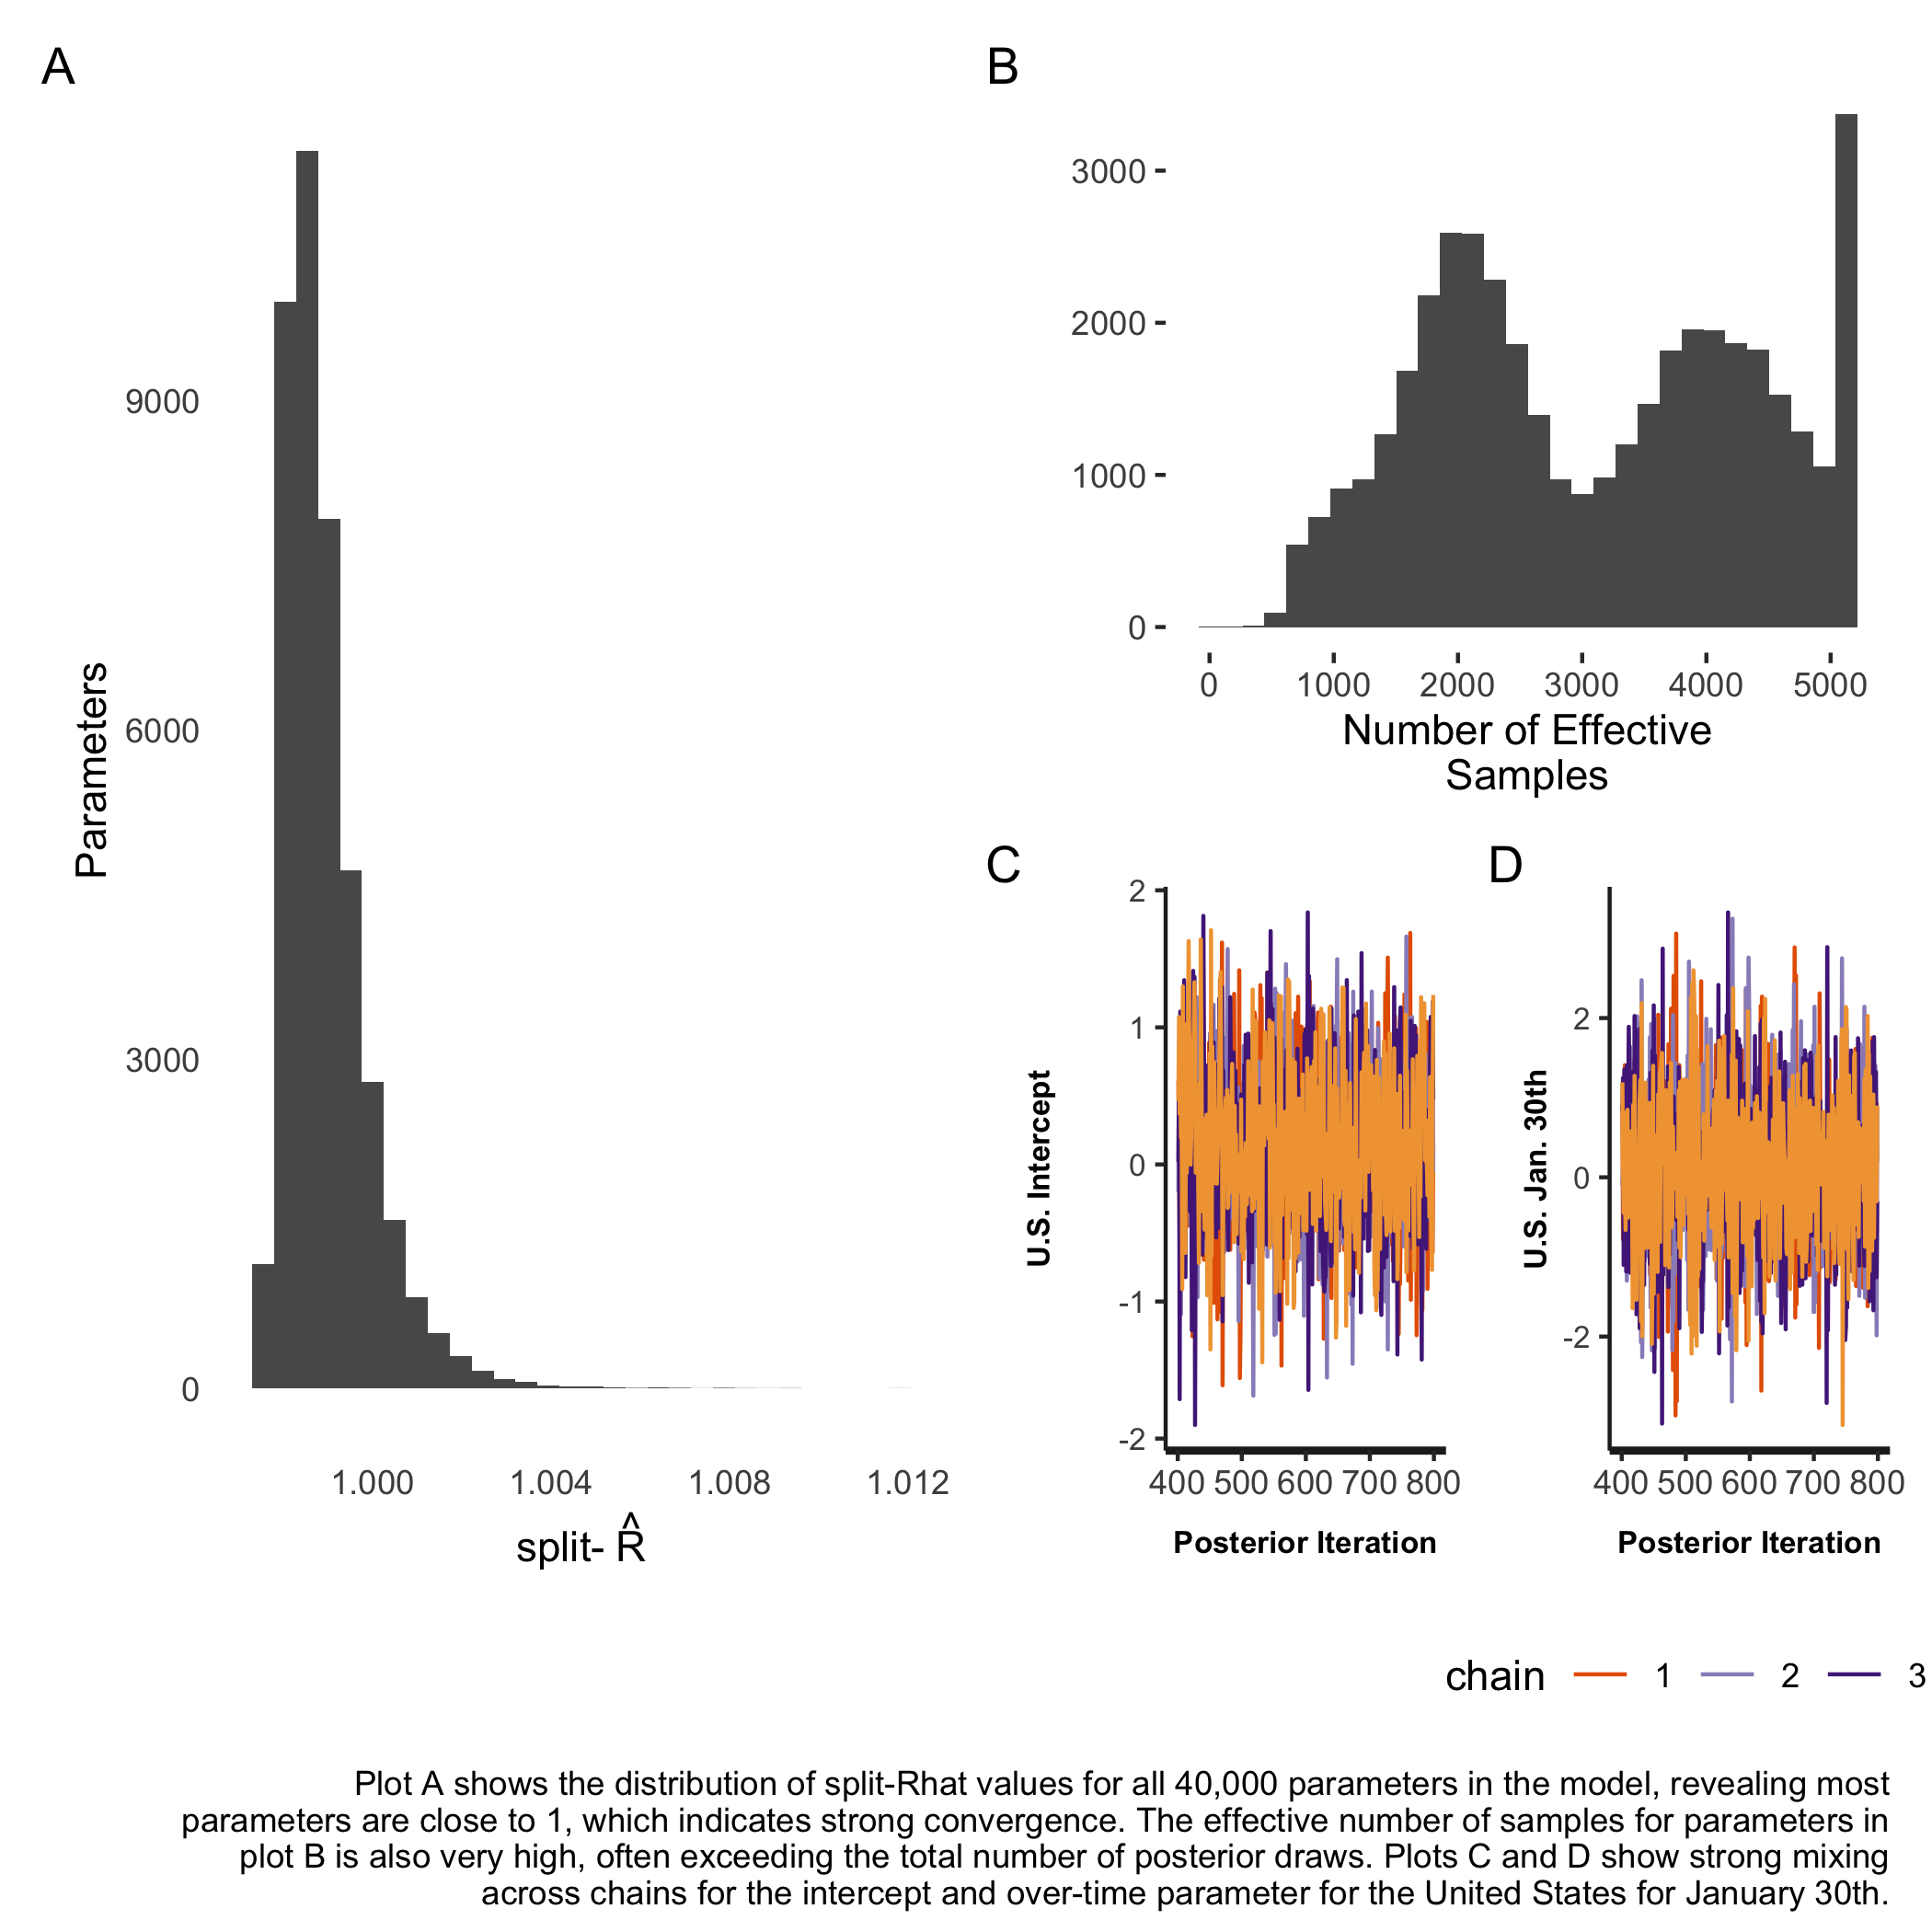
\includegraphics[width=6.5in]{mcmc_evaluate} \caption{Convergence Diagnostics for Random-Walk HMC Fit}\label{fig:modelconv}
\end{figure}

\hypertarget{model-validity}{%
\subsection*{Model Validity}\label{model-validity}}
\addcontentsline{toc}{subsection}{Model Validity}

While employing a measurement model ensures robustness to arbitrary data coding errors, it is still necessary to validate the model's over-time process, which imposes some assumptions on how policy activity scores change over time. The use of a random walk implies that policy differences will be relatively stable from one day to the next, which could limit the ability of scores to encompass quick, discontinuous changes.\textsuperscript{78} While we employ this particular specification because it has been applied previously to a variety of empirical phenomena and because of its relative parsimony, we can partially test for whether it captures changes by estimating a static IRT model for each day in the sample. The corresponding estimates represent cross-sections without any time process imposed.

Due to the complexity of comparing the estimates, we plot the results for six countries separately in Figure \ref{fig:timeest}. This figure shows that indeed the cross-sectional estimates can show much more discontinuous jumps, though we note at the same time that there appears to be substantial noise in the estimates as they only incorporate information available at a single day. Nonetheless, while the random-walk estimates certainly exhibit less discontinuos change, they do still allow for very quick divergence in policy activity scores, with France and Russia moving from the bottom to the top of the index in the space of only a few weeks.

\begin{figure}
\centering
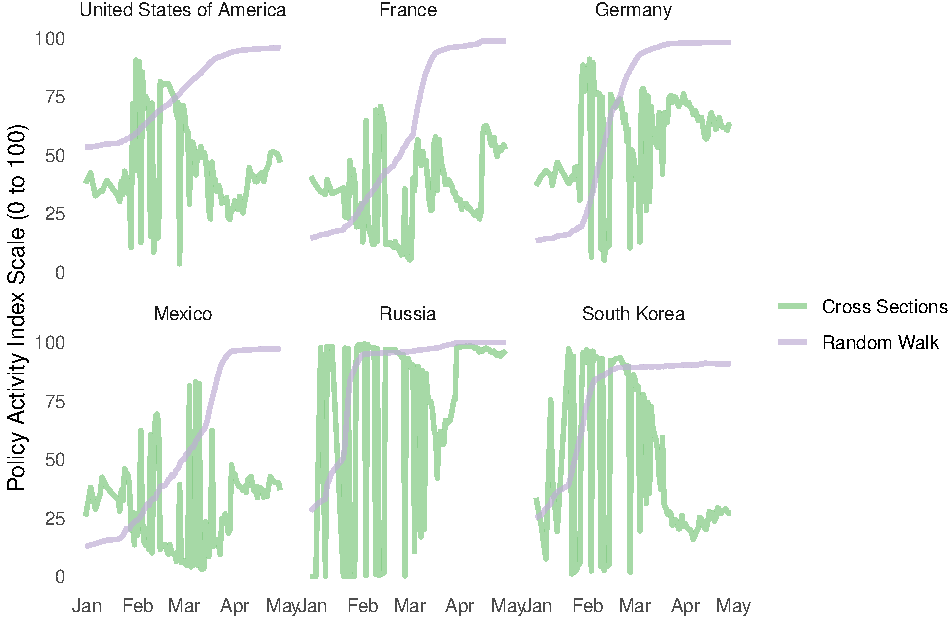
\includegraphics{corona_wp_R1_nature_files/figure-latex/timeest-1.pdf}
\caption{\label{fig:timeest}Comparison of Cross-sectional Estimates of Policy Activity Scores to the Random-Walk Time Series Estimates}
\end{figure}

We note as well that the model is parameterized so that each country has its own variance parameter. This permits the rate of change to vary by country, reducing the concern that the model may be overly restricting change. These variance parameters are shown in Figure \ref{fig:plotvar}, sorted in order of increasing over-time variance. These estimates are themselves substantively interesting, as the United States, which was used as the reference category, has actually one of the lowest rates of over-time change, while some countries like New Zealand, Spain and San Marino witnessed the highest variance in policy activity scores. Because at this time the index only captures increasing numbers of policies, the variance parameters can be given the interpretation of which countries responded in the shortest period of time across a broad array of policy indicators.

\begin{figure}
\centering
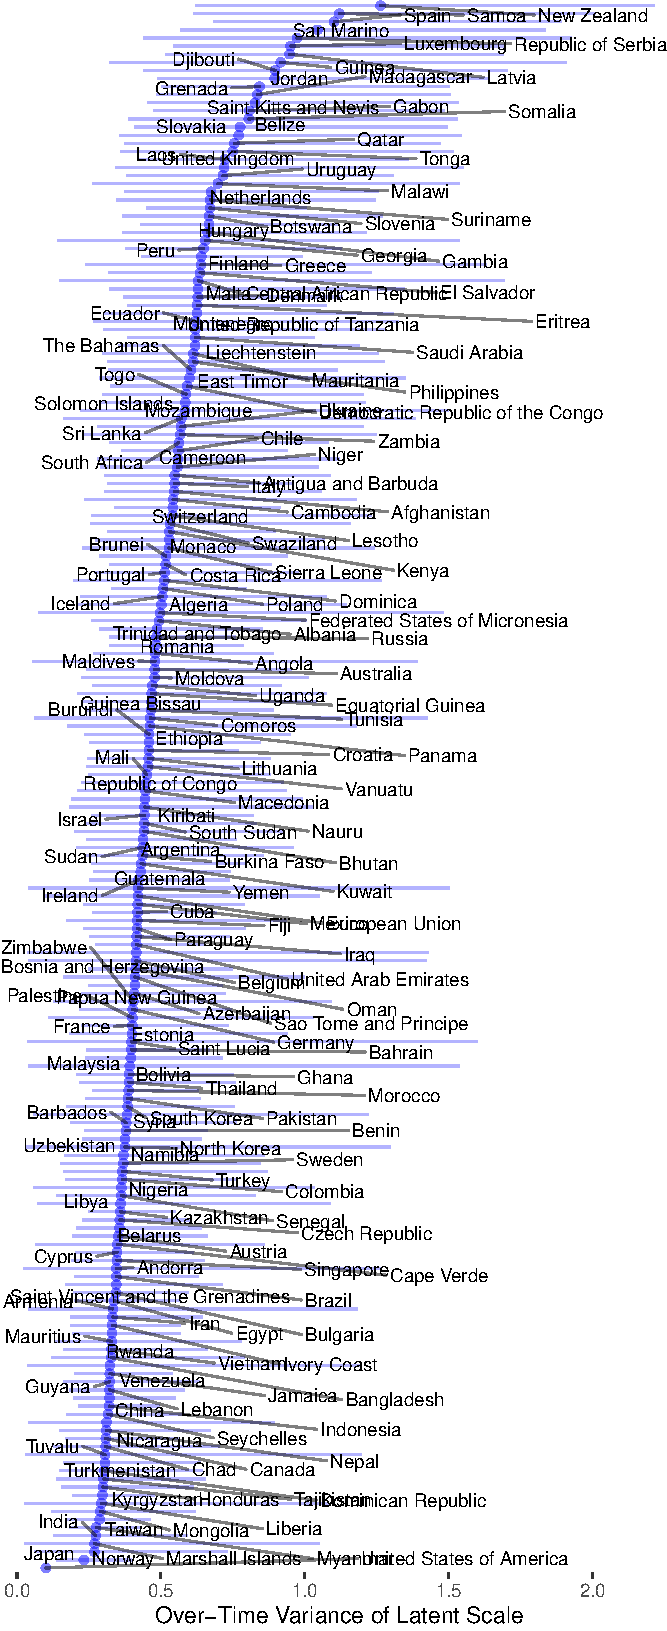
\includegraphics{corona_wp_R1_nature_files/figure-latex/plotvar-1.pdf}
\caption{\label{fig:plotvar}Country-level Variance (Over-time Change) Parameters from Policy Activity Index Estimation}
\end{figure}

\hypertarget{data-schema}{%
\subsection*{Data Schema}\label{data-schema}}
\addcontentsline{toc}{subsection}{Data Schema}

Each policy records at the minimum, the following information: The policy type; the name of the country from which a policy originates. If the policy originates from a province or state, that information is also documented. Future versions of the dataset will also include information on whether a policy was initiated from a city or municipality or another level of government; the degree to which a policy must be complied with; the entity enforcing the policy; The date a policy is announced, implemented and ends. Note that sometimes policies are announced without a pre-determined end date. In those cases, this field is left blank.

For all policies, the database further documents information about the geographic target of the policy and the human or material target of a policy. Note however, for some policies, the geographic target may be the same as the policy initiator and in those cases can be considered monadic. Where applicable, we also document the directional flow of the policy, and the mechanism of travel.

All of the information mentioned above is also provided qualitatively via a textual policy description. Additional meta-data that is available for all policies include when the record entered into the database and a link for the information source for the policy. See the appendix for a list of currently available fields in the data, along with a list of external data variables such as country-level covariates that are added in to daily releases, including COVID-19 tests and cases.

There is a unique record ID for each unique policy announcement, which we code at the policy sub category type. That is, some policy types are further categorized into sub-categories. E.g. `Quarantine' can be further classified into one or more of the following sub categories: `Self-Quarantine', `Government Quarantine', `Quarantine outside the home or government facility', `Quarantine only applies to people of certain ages' and `Other'. Of the 13074 such events in the dataset, we have identified 11052 unique events. That is, some events in the database are updates or changes to existing policies. We link such events over time using a unique ID, which we term the policy ID as opposed to the record ID. An event counts as an update if it deals with a change in either the:

\begin{enumerate}
\def\labelenumi{\arabic{enumi}.}
\tightlist
\item
  Time duration (E.g. A country lengthens its quarantine to 28 days from 14 days.);
\item
  Strength of an existing policy in terms of either:

  \begin{enumerate}
  \def\labelenumii{\alph{enumii}.}
  \tightlist
  \item
    quantitative `amount' of the policy (E.g. A restriction of mass gatherings was previously set at 100 people and now it is set at 50 people)
  \item
    compliance rules for the policy (E.g. The quarantine used to be voluntary but now its mandatory.)
  \item
    who the policy applies towards (E.g. The quarantine used to apply to people of all ages and now it only applies to the elderly.)
  \end{enumerate}
\end{enumerate}

A policy counts as a new entry and not an update if it deals with a change in any other dimension, e.g.~the qualtitative policy type (e.g.~a quarantine used to mandate a stay in a government facility but now quarantine at home is allowed), targeted country (e.g.~quarantine upon arrival was mandated for people traveling from China but now these rules also apply to people traveling from Italy) etc.

\hypertarget{data-collection-methodology}{%
\subsection*{Data Collection Methodology}\label{data-collection-methodology}}
\addcontentsline{toc}{subsection}{Data Collection Methodology}

As researchers learn more about the various health, economic, and social effects of the COVID-19 pandemic, it is crucial that they have access to data that is reliable, valid, and timely (to the greatest extent possible). We have adopted a data collection methodology that we believe optimizes over all three of these constraints.

To collect the data, we recruited more than 260 research assistants (RAs) from colleges and universities around the world, representing 18 out of the 24 time zones.\footnote{For more information on the individual RAs, please visit \url{http://coronanet-project.org/}} Large social scientific datasets typically rely on experts, coders, or crowd-sourcing to input data. The literature has shown that common coding tasks can be completed via crowd-sourcing,\textsuperscript{79,80} but that there are also limitations to the wisdom of crowds when specific contextual or subject knowledge is required.\textsuperscript{81,82} To address these trade offs, we decided to train current students to code our entries, leveraging the benefits of wide-spread recruitment and a diverse pool of country-specific knowledge from across the globe. Data collection started on March 28, 2020 and has proceeded rapidly, reaching 13074 records as of the date of this article. Each RA is responsible for tracking government policy actions for at least one country. RAs were allocated depending on their background, language skills and expressed interest in certain countries.\textsuperscript{83}\footnote{Note depending on the level of policy coordination at the national level, certain countries were assigned multiple RAs, e.g.~the United States, Germany, or France.}

We have also partnered with the machine learning company Jataware to automate the collection of more than 200,000 news articles from around the world related to COVID-19.\footnote{We thank Brandon Rose and Jataware for making the news database available to this project.} Jataware employs a natural language processing (NLP) classifier using Bidirectional Encoder Representations from Transformers (BERT) to detect whether a given article is indicative of a governmental policy intervention related to COVID-19. They then apply a secondary NLP classifier to categorize the type of policy intervention (e.g.~``declaration of emergency'', ``quarantine'', ``travel restrictions'', etc.). Next, Jataware extracts the geospatial and temporal extent of the policy intervention (e.g.~``Washington DC'' and ``March 15, 2020'') whenever possible. The resulting list of news sources is then provided to our RAs as an additional source for manual coding and further data validation.

In what follows, we describe in greater detail how RAs document the policies that they identify using our data collection software instrument, and our post data-collection validation procedure. Please refer to the appendix for more information on our procedure for on-boarding and training RAs and our system for communicating with and organizing RAs.

\hypertarget{data-collection-software-instrument}{%
\subsubsection*{Data Collection Software Instrument}\label{data-collection-software-instrument}}
\addcontentsline{toc}{subsubsection}{Data Collection Software Instrument}

We designed a Qualtrics survey with survey questions about different aspects of a government policy action to streamline the CoronaNet data collection effort. With this tool, RAs can easily and efficiently document different policy actions by answering the relevant questions posed in the survey.\footnote{See 84 for an example of a similar use of Qualtrics in collecting data.} For example, instead of entering the country that initiated a policy action into a spreadsheet, RAs answer the following question in the survey: ``From what country does this policy originate?'' and choose from the available options given in the survey.

By using a survey instrument to collect data, we are able to systematize the collection of very fine-grained data while minimizing coding errors common to tools like shared spreadsheets. The value of this approach of course, depends on the comprehensiveness of the questions posed in the survey, especially in terms of the universe of policy actions that countries have implemented against COVID-19. For example, if the survey only allowed RAs to select `quarantines' as a government policy, it would not capture any data on `external border restrictions', which would seriously reduce the value of the resulting data.

As such, to ensure the comprehensiveness of the data, before designing the survey, we collected in depth, over-time data on policy actions taken by one country, Taiwan, since the beginning of the outbreak as well as cross-national data on travel bans implemented by most countries for a total of 245 events.\footnote{The specific data source we cross referenced for this effort was the March 20, 2020 version of the following New York Times article: Salcedo, Andrea and Gina Cherelus, ``Coronavirus Travel Restrictions, Across the Globe'' \emph{New York Times}, 20 March 2020, \url{https://www.nytimes.com/article/coronavirus-travel-restrictions.html}} We chose to focus on Taiwan on because of its relative success, as of March 28, 2020, in limiting the negative health consequences of COVID-19 within its borders.\footnote{Beech, Hannah. ``Tracking the Coronavirus: How Crowded Asian Cities Tackled an Epidemic.'' \emph{New York Times} 18 March 2020, \url{https://www.nytimes.com/2020/03/17/world/asia/coronavirus-singapore-hong-kong-taiwan.html}} As such, it seems likely that other countries may choose to emulate some of the policy measures that Taiwan had implemented, which helps increase the comprehensiveness of the questions we ask in our survey. Meanwhile, by also investigating variation in how different countries around the world have implemented travel restrictions, we have also helped ensure that our survey is able to comprehensively document variation in how an important and commonly used policy tool is applied, e.g., restrictions on different methods of travel (e.g.~flights, cruises), restrictions across borders and within borders, restrictions targeted toward people of different status (e.g.~citizens, travelers).

There are many additional benefits of using a survey instrument for data collection, especially in terms of ensuring the reliability and validity of the resulting data:

\begin{enumerate}
\def\labelenumi{\arabic{enumi}.}
\item
  Preventing unforced measurement error. RAs are prevented from entering data into incorrect fields or unknowingly overwriting existing data---as would be possible with manual data entry into a spreadsheet---because RAs can only document one policy action at a time in a given iteration of a survey and do not have access to the full spreadsheet when they are entering in the data.
\item
  Standardizing responses. We are able to ensure that RAs can only choose among standardized responses to the survey questions, which increases the reliability of the data and also reduces the likelihood of measurement error. For example, when RAs choose different dates that we would like them to document (e.g., the date a policy was announced) they are forced to choose from a calendar embedded into the survey which systematizes the day, month and year format that the date is recorded in.
\item
  Minimizing measurement error. A survey instrument allows coding different conditional logics for when certain survey questions are posed. This technique obviates the occurrence of logical fallacies in our data. For example, we are able to avoid situations where an RA might accidentally code the United States as having closed all schools in another country.
\item
  Reduction of missing data. We are able to reduce the amount of missing data in the dataset by using the forced response option in Qualtrics. Where there is truly missing data, there is a text entry at the end of the survey where RAs can describe what difficulties they encountered in collecting information for a particular policy event.
\item
  Reliability of the responses. We increase the reliability of the documentation for each policy by embedding descriptions of different possible responses within the survey. For example, in the survey question where RAs are asked to identify the policy type (\texttt{type} variable, see appendix and/or Codebook), the survey question includes pop-up buttons which allow RAs to easily access descriptions and examples of each possible policy type. Such pop-up buttons were also made available for the survey questions which code for the people or materials a policy was targeted at (\texttt{target\_who\_what}) and whether the policy was inbound, outbound or both (\texttt{target\_direction}). Embedding such information in the dataset both clarifies the distinction between different answer choices and increases the efficiency of the policy documentation process (as RAs are not obliged to refer back and forth from the survey to the codebook).
\item
  Linking observations. The use of a survey instrument allows us to easily link policy events together over time should there be updates to existing policies. Once coded, each policy is given a unique Record ID, which RAs can easily look up, reference and link to if they need to update a particular policy.
\end{enumerate}

\hypertarget{post-data-collection-validation-checks}{%
\subsubsection*{Post-Data Collection Validation Checks}\label{post-data-collection-validation-checks}}
\addcontentsline{toc}{subsubsection}{Post-Data Collection Validation Checks}

We further implement the following processes to validate the quality of the dataset:

\begin{enumerate}
\def\labelenumi{\arabic{enumi}.}
\item
  Cleaning. Before validation, we use a team of RAs to check the raw data for logical inconsistencies and typographical errors.
\item
  Multiple Coding for Validation. Others have shown that the random allocation of tasks and the validation of labels by more than one coder are among the best ways to improve the quality of a dataset.\textsuperscript{85,86} We randomly sample 10\% of the dataset using the source of the data (e.g.~newspaper article, government press release) as our unit of randomization. We use the source as our unit of randomization because one source may detail many different policy types. We then provide this source to a fully independent RA and ask her to code for the government policy contained in the sampled source in a separate, but identical, survey instrument. If the source is in a language the RA cannot read, then a new source is drawn. The RA then codes all policies in the given source. This practice is repeated a third time by a third independent coder. Given the fact that each source in the sample is coded three times, we can assess the reliability of our measures and report the reliability score of each coder.
\item
  Evaluation and Reconciliation. We then check for discrepancies between the originally coded data and the second and third coding of the data through two primary methods. First, we use majority-voting to establish a consensus for policy labels. Using the majority label as an estimate of the ``hidden true label'' is a common method to address classification problems.\textsuperscript{87} One issue with this approach is that it assumes that all coders are equally competent.\textsuperscript{88} This criticism is generally levied at data creation with crowd-sourced laborers. We mitigate this problem by training our RAs in the data collection process and prioritizing RA country-knowledge and language skills, therefore ensuring a more equal baseline for RA quality. In addition, we provide RA ID codes that will allow users to evaluate coder accuracy.
\end{enumerate}

If the majority achieves consensus, then we consider the entry valid. If a discrepancy exists, a fourth RA or PI evaluates between the three entries to determine whether one, some, a combination of all three is most accurate. Reconciled policies are then entered into the dataset as a correction for full transparency. If an RA was found to have made a coding mistake, then we sample six of their previous entries: 3 entries which correspond to the type of mistake made\footnote{e.g.~if the RA incorrectly codes an `External Border Restriction' as a `Quarantine', we sample 3 entries where the RA has coded a policy as being about a `Quarantine.'} and randomly sample 3 more entries to ascertain whether the mistake was systematic or not. If systematic errors are found, entries coded by that individual will be entirely recoded by a new RA.

At the time of writing, we are in the process of completing our second coding of the validation sample. Thus far, 297 policies have been double coded---276 double-coded policies after excluding the category `Other policies' from the analysis---out of the original 500 randomly-selected policies included in our validation set. This is equivalent to 10\% of the first 5,000 policies in the dataset. We will be gradually expanding the validation set until we cover all observations.

We provide several measures in Table \ref{tab:validation} to evaluate the inter-coder reliability at this early stage of validation. We find remarkable heterogeneity in the inter-coder reliability across types of policies. Our coders show a substantial level of agreement on policies such as `Restrictions of Mass Gatherings' (n = 21, k = 0.95), `Closure of Schools' (n = 14, k = 0.92), `Restrictions of Non-Essential' (n = 19, k = 0.89), `External Border Restrictions' (n = 52, k = 0.83), `Curfew' (n = 6, k = 0.82), and Internal Border Restrictions (n = 11, k = 0.80). However, we also observe poor inter-rater agreement scores in other policies such as `Social Distancing' (n = 14, k = 0.38), `Public Awareness Measures' (n = 15, k = 0.49), and `New Task Force, Bureau or Administrative Configuration' (n = 9, k = 0.52). Overall, these statistics indicate substantial levels of overall agreement between coders with inter-coder reliability scores between 0.71 and 0.74 (n = 276).

Our initial assessment of miscodings suggests that `Quarantine/Lockdowns' and `Social Distancing' policies are conceptually difficult to distinguish for our coders. To ameliorate this issue, we have recently separated Quarantine from Lockdowns and added branching logic into the Qualtrics survey that also clarifies the specific sub-policies that fall under `Quarantine', `Lockdowns', and `Social Distancing'. Additionally, our coders often fail to distinguish between `Public Awareness Campaigns' and `Social Distancing' policies. Our recent survey additions add several sub-types of `Public Awareness Campaigns' that should conceptually clarify these policies. Further, the creation of a `New Task Force, Bureau or Administrative Configuration' often goes together with a number of additional policies. In these cases, some of our coders seem to focus on these additional policies rather than on the creation of administrative units, which lowers the reliability of the coding system for this policy. Finally, we have detected extremely poor reliability for the health-related policies of `Health Monitoring' and `Health Testing'. We have clarified the distinction across the three health-related policies---namely, `Health Resources', `Health Monitoring' and `Health Testing'---in the codebook and we combine them under the category of `Health Measures' in this on-going validation.

In the following weeks, we expect inter-coder reliability scores to improve as a consequence of three processes: (a) coders acquire more experience with the codebook and the coding task in general; (b) we clean the dataset of obvious errors and logical inconsistencies; and, (c) we keep clarifying and improving the codebook and the coding system. Notwithstanding these processes, we acknowledge that some ambiguities will unavoidably remain providing evidence for the utility of our planned ``majority voting'\,' validation strategy.

\begin{table}[!h]
\centering
\caption{Inter-Coder Reliability Measures for On-Going Validation}
\label{tab:validation}
\resizebox{\textwidth}{!}{%
\begin{tabular}{lccc}
\hline
\textbf{Policy} & \multicolumn{1}{c}{\textbf{(n)}} & \multicolumn{1}{c}{\textbf{Percentage Agreement}} & \multicolumn{1}{c}{\textbf{Cohen's Kappa (k)}} \\ \hline
Restrictions of Mass Gatherings & 21 & 95.2 & 0.95 \\
Closure of Schools & 14 & 92.9 & 0.92 \\
Restriction of Non-Essential Businesses & 19 & 89.5 & 0.89 \\
External Border Restrictions & 52 & 84.6 & 0.83 \\
Curfew & 6 & 83.4 & 0.82 \\
Internal Border Restrictions & 11 & 81.8 & 0.80 \\
Declaration of National Emergency & 19 & 73.7 & 0.71 \\
Quarantine/Lockdown & 28 & 67.9 & 0.65 \\
Health Measures & 52 & 65.4 & 0.63 \\
Restriction of Non-Essential Government Services & 16 & 62.5 & 0.59 \\
New Task Force, Bureau or Administrative Configuration & 9 & 55.6 & 0.52 \\
Public Awareness Measures & 15 & 53.3 & 0.49 \\
Social Distancing & 14 & 42.9 & 0.38 \\
 &  &  &  \\
 \hline
 \hline
 &  &  &  \\
\textbf{Summary Inter-coder Reliability Scores} &  &  &  \\
Percentage Agreement & \multicolumn{1}{c}{0.74} & &  \\
Cohen's Kappa & \multicolumn{1}{c}{0.72} & & \multicolumn{1}{l}{} \\
Krippendorff's alpha & \multicolumn{1}{c}{0.71} & & \multicolumn{1}{l}{} \\
Scott's PI -- Estimate (SE) & \multicolumn{1}{c}{0.71 (0.03)} & & \\ 
 &  & & \\
\hline \hline
\end{tabular}
}
\end{table}

\hypertarget{conclusion}{%
\section*{Conclusion}\label{conclusion}}
\addcontentsline{toc}{section}{Conclusion}

As policymakers, researchers and the broader public debate and compare how to succeed against the novel threats posed by COVID-19, they need real-time, traceable data on government policies in order to understand which of these policies are effective, and under what conditions. This requires specific knowledge of the variation in such policies and the extent of their implementation across countries and time. The goal of the dataset and policy action index presented here is to provide this information.

We have tried to match our data collection efforts to keep up with the exponential speed with which COVID-19 has already upended global public health and the international economy while also maintaining high levels of quality. However, we will inevitably be refining, revising and updating our data to reflect new knowledge and trends as the pandemic unfolds. The data that we present in this first version of the dataset represents only the initial release of the data, and we will continue to validate and release data so long as governments continue to develop policies in response to COVID-19.

In future work, we intend to analyze the policy combinations that are best able to stymie the epidemic so as to contribute to the research community and provide urgently needed knowledge for policymakers and the wider global public.

\newpage

\hypertarget{data-availability}{%
\subsection*{Data Availability}\label{data-availability}}
\addcontentsline{toc}{subsection}{Data Availability}

For the most current, up to date version of the dataset, please visit \url{http://coronanet-project.org} or our Github page at \url{https://github.com/saudiwin/corona_tscs}.

Interested readers may also find our code for collecting the data and maintaining the database at the aforementioned Github page. For more information on the exact variables collected, please see our publicly available \href{https://docs.google.com/document/d/1zvNMpwj0onFvUZ_gLl4RRjqS-clbHv3TIX6EOHofsME/edit?usp=sharing}{codebook here} and visit our \href{https://coronanet-project.org/}{website}.

\hypertarget{code-availability}{%
\subsection*{Code Availability}\label{code-availability}}
\addcontentsline{toc}{subsection}{Code Availability}

Interested readers may also find our code for collecting the data and maintaining the database at our Github page: \url{https://github.com/saudiwin/corona_tscs}.

\hypertarget{acknowledgements}{%
\subsection*{Acknowledgements}\label{acknowledgements}}
\addcontentsline{toc}{subsection}{Acknowledgements}

We thank the very large number of research assistants who coded this data. Their affiliations and vita are listed in the appendix. Our research assistants include:
Abdelaziz Ibn Abdelouahab, Abhyudaya Tyagi, Adriana Poppe, Advait Arya, Alette Mengerink, Alexander Pachanov, Alexandra Michaelsen, Alisa Udodik, Amadeus Albrecht, Amanda Panella, Ana Acero, Anabella McElroy, Anastasia Steinbrunner, Andreas Duncan, Andres Lopez Schrader, Anelia Petrova, Angad Johar, Angela Herz, Angeline Kanyangi, Anke Horn, Anna Sophia Körner, Annika Kaiser, Anoushka Thakre, Antonia Pérez, Ariana Barrenechea, Arianna Schouten, Avery Edelman, Aysina Maria, Babrik Kushwaha, Barbora Bromová, Beatrice Di Giulio, Beatrice von Braunschweig, Bianca Grizhar, Borja Arrue-Astrain, Brahim Ouerghi, Brian Chesney Quartey, Bruno Ciccarini, Calvin Kaleel, Cara Kim, Caress Schenk, Carl Philip Dybwad, Carlos Velez, Carly Kimmett, Carmen Alija, Caroline Beale, Charlotte Vorbauer, Cheng-Hao Shen, Chloë Fraser, Cornelia Marie Dybwad, Cory Martin, Csilla Horvath, Dan Downes, Dan Wu, Daniel Boey, Daniel Martínek, Dariga Abilova, Davit Jintcharadzé, Deborah Agboola, Dick Paul Ouko, Diego Calvo, Dominik Juling, Donia Kamel, Dorian Quelle, Dotrus Wilstic, Dovile Jankunaite, Dr Michelle King-Okoye, Dylan Ollivier, Eduardo Landaeta, Elaine Lin, Elfriede Derrer-Merk, Elisa Seith, Elizabeth (Lizzie) Jones, Ella Pettersen, Elliot Weir, Emma Hutchinson, Esther Ollivier, Eugene Kwizera, Fabienne Lind, Fabio Kadner, Fadhilah Fitri Primandari, Farah Sadek, Feifei Wang, Felix Willuweit, Fernanda Werneck, Francis Yoon, Frank Yuxuan Sun, Franziska Nguyen, Frederic Denker, Gloria Mutheu, Godfrey Katiambo, Griffyne Makaoko, Ha-Neul Yu, Hafsa Ahmed, Hajar Chams Eddine, Helene Paul, Helwan Felappi, Heman Asibuo, Henry Okwatch, Ilona Koch, Imogen Rickert, Ines Böhret, Ingeborg Sæle Helland, Ingrid Ravnanger, Isabela Russo, Isabelle Smith, Ismail Jamai Ait Hmitti, Jack Kubinec, Jakob Berg, Jane Murutu, Janet Li, Janice Klaiber, Janne Luise Piper, Jasmina Sowa, Jean von Agris, Jennifer Noguera Barrera, Jessica Johansson, Jiho Yoo, Joana Lencastre Morais, Joel Gräff, Josef Montag, Jule Scholten, Julia Dröge, Julia Nassl, Julia Smakman, Julia Wießmann, Kadriye Nisa Başkan, Karina Lisboa Båsund, Karlotta Schultz, Katharina Klaunig, Kayla Schwoerer, Khoa Tran, Klea Vogli, Kojo Vandyck, Konstanze Schönfeld, Laura Cadena, Laura Williamson, Laureen Hannig, Laurent Frick, Lea Clara Frömchen-Zwick, Lea Wiedmann, Lena Kolb, Leon Kohrt, Leonie Imberger, Li Cheng, Lilli Tabea Albrecht, Lily Zandstra, Lincoln Dow, Linlin Chen, Luise Modrakowski, Lya Cuéllar, Magdalena Strebling, Maheen Zahra, Maira Sheikh, Maisa Nasirova, Maite Spel, Malina Winking, Mamle Akosua Kwao, Mara Förster, Marianne Sievers, Marius Deierl, Marlies Hofmann, Mary Nussbaumer, Maryam AlHammadi, Mascha Hotopp, Mats Jensen, Matthew Cottrell, Matthew Hargreaves, Matthew Tan, Maximilian Dirks, Maya Rollberg, Maya Sugden, Mehdi Bhouri, Michaela Balluff, Milan Chen, Milos Moskovljevic, Miranda Tessore Janowski, Miriam Witte, Mirjam Muller, Mona Horn, Muhammad Masood, Muhannad Alramlawi, Museera Moghis, Mustafa Nasery, Nadja Grossenbacher, Natalia Filkina-Spreizer, Nathan Ruhde, Nicolas Göller, Nicole Oubre, Nida Hasan, Niklas Illenseer, Nikolina Klatt, Nivedita Darshini Bholah, Noah Fröhlich, Noelle Kubinec, Noor Altunaiji, Océane Mauffrey, Oketch Juliet Anyango, Oliver Pollex, Oliver Weber, Olzhas Gibatov, Omer Syed, Ongun Durhan, Oscar Courtier, Pablo Robles, Paula Germana, Philipp Weber, Pia Bansagi, Racha Hanine, Rachel Dada, Rahman Demirkol, Raquel Karl, Rebecca Beigel, Ricardo Buitrago, Richmond Silvanus Baye, Robin Fischer, Rosana Fayazzadh, Saif Khan, Salma Soliman, Samantha Law, Samantha Reinard, Sana Moghis, Sarah Edmonds, Sarah Sleigh, Sau Kan Chan, Saw Eh Doh Soe, Sean-Michael Pigeon, Seung-A Paik, Shalini Corea, Shruti Shukla, Simon Hüttemann, Sonja Müller, Sophia Tomany, Stefanie Mallow, Stella Dold, Su Ülkenli, Surendra Belbase, Symrun Razaque, Tanja Matheis, Tara Goodsir, Tasia Wagner, Temur Davronov, Tess de Rooij, Tess Martin, Tilda Nilsson Gige, Tom Seiler, Tristan Brömsen, Ugochukwu Okoye, Ursela Barteczko, Vellah Kedogo Kigwiru, Veronica Velasquez Mesa, Veronika Bartáková, Victor Abuor, Victoria Atanasov, Vida Han, Vinayak Rajesekhar, Winrose Njuguna, Xian Jin, Yifei Zhu, Yoes C. Kenawas, Zhandos Ybrayev.

We also thank Tim Büthe, the Chair for International Relations, the Hochschule für Politik at the Technical University of Munich (TUM), the TUM School of Governance, and the TUM School of Management for the many ways he has supported this project. We further thank New York University Abu Dhabi for funding in support of this endeavor. Moreover, we appreciate the support by Slack Technologies and RStudio Inc.~who provided access to their technical infrastructure.

\hypertarget{competing-interests}{%
\subsection*{Competing interests}\label{competing-interests}}
\addcontentsline{toc}{subsection}{Competing interests}

The authors declare no competing interests.

\hypertarget{appendix-a-description-of-dataset-fields}{%
\subsection*{Appendix A: Description of Dataset Fields}\label{appendix-a-description-of-dataset-fields}}
\addcontentsline{toc}{subsection}{Appendix A: Description of Dataset Fields}

The format of the data is in country-day-\texttt{record\_id} format. Some \texttt{record\_id} values have letters appended to indicate that the general policy category \texttt{type} also has a value for \texttt{type\_sub\_cat}, which contains more detail about the policy, such as whether health resources refers to masks, ventilators, or hospitals. Some entries are marked as \texttt{new\_entry} in the \texttt{entry\_type} field for when a policy of that type was first implemented in the country. Later updates to those policies are marked as updates in \texttt{entry\_type}. To see how policies are connected, look at the \texttt{policy\_id} field for all policies from the first entry through updates for a given country/province/city. If an entry was corrected after initial data collection, it will read corrected in the \texttt{entry\_type} field (the original incorrect data has already been replaced with the corrected data).

\begin{enumerate}
\def\labelenumi{\arabic{enumi}.}
\item
  \textbf{\texttt{coronanet\_release.csv}} This file contains variables from the CoronaNet government response project, representing national and sub-national policy event data from more than 190 countries since December 31st, 2019. The data include source links, descriptions, targets (i.e.~other countries), the type and level of enforcement, and a comprehensive set of policy types. For more detail on this data, you can see our \href{https://docs.google.com/document/d/1zvNMpwj0onFvUZ_gLl4RRjqS-clbHv3TIX6EOHofsME}{codebook here}.
\item
  \textbf{\texttt{coronanet\_release\_allvars.csv}} This file contains the government response information from \texttt{coronanet\_release.csv} along with the following datasets:

  \begin{enumerate}
  \def\labelenumii{\alph{enumii}.}
  \tightlist
  \item
    Tests from the CoronaNet testing database (See \url{http://coronanet-project.org} for more info);
  \item
    Cases/deaths/recovered from the \href{https://github.com/CSSEGISandData/COVID-19}{JHU data repository};
  \item
    Country-level covariates including GDP, V-DEM democracy scores, human rights indices, power-sharing indices, and press freedom indices from the \href{https://niehaus.princeton.edu/news/world-economics-and-politics-dataverse}{Niehaus World Economics and Politics Dataverse}
  \end{enumerate}
\end{enumerate}

\hypertarget{coronanet_release.csv-field-dictionary}{%
\subsection*{\texorpdfstring{\texttt{coronanet\_release.csv} Field Dictionary}{coronanet\_release.csv Field Dictionary}}\label{coronanet_release.csv-field-dictionary}}
\addcontentsline{toc}{subsection}{\texttt{coronanet\_release.csv} Field Dictionary}

\begin{enumerate}
\def\labelenumi{\arabic{enumi}.}
\tightlist
\item
  \texttt{record\_id} Unique identifier for each unique policy record
\item
  \texttt{policy\_id} Identifier linking new policies with subsequent updates to policies
\item
  \texttt{recorded\_date} When the record was entered into our data
\item
  \texttt{date\_announced} When the policy is announced
\item
  \texttt{date\_start} When the policy goes into effect
\item
  \texttt{date\_end} When the policy ends (if it has an explicit end date)
\item
  \texttt{entry\_type} Whether the record is new, meaning no restriction had been in place before, or an update (restriction was in place but changed). Corrections are corrections to previous entries.
\item
  \texttt{event\_description} A short description of the policy change
\item
  \texttt{type} The category of the policy
\item
  \texttt{type\_sub\_cat} The sub-category of the policy (if one exists)
\item
  \texttt{type\_text} Any additional information about the policy type (such as the number of ventilators/days of quarantine/etc.)
\item
  \texttt{country} The country initiating the policy
\item
  \texttt{init\_country\_level} Whether the policy came from the national level or a sub-national unit
\item
  \texttt{province} Name of sub-national unit
\item
  \texttt{target\_country} Which foreign country a policy is targeted at (i.e.~travel policies)
\item
  \texttt{target\_geog\_level} Whether the target of the policy is a country as a whole or a sub-national unit of that country
\item
  \texttt{target\_region} The name of a regional grouping (like ASEAN) that is a target of the policy (if any)
\item
  \texttt{target\_province} The name of a province targeted by the policy (if any)
\item
  \texttt{target\_city} The name of a city targeted by the policy (if any)
\item
  \texttt{target\_other} Any geographical entity that does not fit into the targeted categories mentioned above
\item
  \texttt{target\_who\_what} Who the policy is targeted at
\item
  \texttt{target\_direction} Whether a travel-related policy affects people coming in (Inbound) or leaving (Outbound)
\item
  \texttt{travel\_mechanism} If a travel policy, what kind of transportation it affects
\item
  \texttt{compliance} Whether the policy is voluntary or mandatory
\item
  \texttt{enforcer} What unit in the country is responsible for enforcement
\item
  \texttt{link} A link to at least one source for the policy
\item
  \texttt{ISO\_A3} 3-digit ISO country codes
\item
  \texttt{ISO\_A2} 2-digit ISO country codes
\end{enumerate}

\hypertarget{coronanet_release_allvars.csv-field-dictionary}{%
\subsection*{\texorpdfstring{\texttt{coronanet\_release\_allvars.csv} Field Dictionary}{coronanet\_release\_allvars.csv Field Dictionary}}\label{coronanet_release_allvars.csv-field-dictionary}}
\addcontentsline{toc}{subsection}{\texttt{coronanet\_release\_allvars.csv} Field Dictionary}

\begin{enumerate}
\def\labelenumi{\arabic{enumi}.}
\item
  All of the fields listed above, plus
\item
  \texttt{tests\_daily\_or\_total} Whether a country reports the daily count of tests a cumulative total
\item
  \texttt{tests\_raw} The number of reported tests collected from host country websites or media reports
\item
  \texttt{deaths} The number of COVID-19 deaths, aggregated to the country-day level (JHU CSSE data)
\item
  \texttt{confirmed\_cases} The number of confirmed cases of COVID-19, aggregated to the country-day level (JHU CSSE data)
\item
  \texttt{recovered} The number of recoveries from COVID-19, aggregated to the country-day level (JHU CSSE data)
\item
  \texttt{ccode} The Correlates of War country code
\item
  \texttt{ifs} IMF IFS country code
\item
  \texttt{Rank\_FP} (most recent year available from Niehaus dataset) Reporters without Borders Press Freedom Annual Ranking
\item
  \texttt{Score\_FP} (most recent year available from Niehaus dataset) Reporters with Borders Press Freedom Score
\item
  \texttt{state\_IDC} (most recent year available from Niehaus dataset) State/Provincial Governments Locally Elected
\item
  \texttt{muni\_IDC} (most recent year available from Niehaus dataset) Municipal Governments Locally Elected
\item
  \texttt{dispersive\_IDC} (most recent year available from Niehaus dataset) Dispersive Powersharing
\item
  \texttt{constraining\_IDC} (most recent year available from Niehaus dataset) Constraining Powersharing
\item
  \texttt{inclusive\_IDC} (most recent year available from Niehaus dataset) Inclusive powersharing
\item
  \texttt{sfi\_SFI} (most recent year available from Niehaus dataset) State fragility index
\item
  \texttt{ti\_cpi\_TI} (most recent year available from Niehaus dataset) Corruption perceptions index
\item
  \texttt{pop\_WDI\_PW} (most recent year available from Niehaus dataset) World Bank population
\item
  \texttt{gdp\_WDI\_PW} (most recent year available from Niehaus dataset) World Bank GDP (total)
\item
  \texttt{gdppc\_WDI\_PW} (most recent year available from Niehaus dataset) World Bank GDP per capita
\item
  \texttt{growth\_WDI\_PW} (most recent year available from Niehaus dataset) World Bank GDP growth percent
\item
  \texttt{lnpop\_WDI\_PW} (most recent year available from Niehaus dataset) Log of World Bank population
\item
  \texttt{lngdp\_WDI\_PW} (most recent year available from Niehaus dataset) Log of World Bank GDP
\item
  \texttt{lngdppc\_WDI\_PW} (most recent year available from Niehaus dataset) Log of World Bank GDP per capita
\item
  \texttt{disap\_FA} (most recent year available from Niehaus dataset) 3 category, ordered variable for disappearances index
\item
  \texttt{polpris\_FA} (most recent year available from Niehaus dataset) 3 category, ordered variable for political imprisonment index
\item
  \texttt{latentmean\_FA} (most recent year available from Niehaus dataset) the posterior mean of the latent variable index for human rights protection)
\item
  \texttt{transparencyindex\_HR} (most recent year available from Niehaus dataset) Transparency Index
\item
  \texttt{EmigrantStock\_EMS} (most recent year available from Niehaus dataset) Total emmigrant stock from
\item
  \texttt{v2x\_polyarchy\_VDEM} (most recent year available from Niehaus dataset) Electoral democracy index
\item
  \texttt{news\_WB} (most recent year available from Niehaus dataset) Daily newspapers (per 1,000 people)
\end{enumerate}

\hypertarget{appendix-b-research-assistant-training-and-management}{%
\subsection*{Appendix B: Research Assistant Training and Management}\label{appendix-b-research-assistant-training-and-management}}
\addcontentsline{toc}{subsection}{Appendix B: Research Assistant Training and Management}

\hypertarget{ra-training}{%
\subsection{RA Training}\label{ra-training}}

All RAs watch a mandatory 50 minute video training of the survey instrument which explains how to use the survey instrument. RAs are also provided with written guidelines on how to collect data and a comprehensive codebook. To briefly describe it here, the written guidelines provide a definition of what counts as a new or updated policy (see Data section for more details) and provides a checklist for RAs to follow in order to identify and document different policies. In the checklist, RAs are instructed to find policies by checking the sources in the order given in the guidelines to identify policies, to document the relevant information into the survey and to save and upload a document of the source they found for each policy into Qualtrics. The codebook meanwhile provides descriptions and examples of the different possible response options in the survey. Using a training video and the written codebook also has the added benefit of helping us efficiently disseminate the information RAs need to use the survey experiment consistently.

In order to participate as an RA in this project, RAs must fill out a form\footnote{See here for the \href{https://docs.google.com/forms/d/e/1FAIpQLSeybAW0DC0UE1x2EqLiTifVFuSUxqJLGFB8VI4wVCG61tVYKg/viewform}{link to the form}.} in which:

\begin{itemize}
\tightlist
\item
  They identify themselves.
\item
  They certify that they have viewed the training video in which we explain how to use the survey instrument.
\item
  They certify they have joined the CoronaNet Slack Channel (see section below for more information).
\item
  They certify that they understand that RA responsibilities entail

  \begin{itemize}
  \tightlist
  \item
    gathering historical data on COVID-19 government policy actions for their country, and;
  \item
    providing daily updates for new government policy actions.
  \end{itemize}
\item
  They certify that they understand they can access the data collection guidelines and codebook or pose their questions on the Slack Channel.
\item
  They certify that they are expected to upload .pdfs of the sources they access to the survey instrument.
\end{itemize}

Once the RA submits the form, they are sent a personalized link to access the survey. With the customized link, we are also able to keep track of which RA coded what entries.

\hypertarget{real-time-communication-and-feedback}{%
\subsection{Real-Time Communication and Feedback}\label{real-time-communication-and-feedback}}

Once an RA joins the project, they can pose their questions on a CoronaNet Slack channel, which they must join in order to participate in the project. The channel allows any RA to pose a question or issue they may have in using the survey instrument to any of the PIs and allows all other RAs to learn from the exchange at the same time. As such, RAs are able to receive feedback and learn from each other's questions in a timely and centralized manner. Since the data collection effort was launched on March 28, 2020 until April 18, 2020, both RAs and PIs have actively used Slack to communicate with one another. On the Slack channel devoted to asking questions about the Qualtrics data survey in particular, there were 1,752 messages posted by 130 project members.

\hypertarget{appendix-c-list-of-contributors-to-dataset}{%
\subsection*{Appendix C: List of Contributors to Dataset}\label{appendix-c-list-of-contributors-to-dataset}}
\addcontentsline{toc}{subsection}{Appendix C: List of Contributors to Dataset}

\begin{longtable}[t]{l>{\raggedright\arraybackslash}p{2cm}>{\raggedright\arraybackslash}p{2cm}>{\raggedright\arraybackslash}p{3cm}}
\caption{\label{tab:ratable}Contributing Researchers and their Responsible Countries}\\
\toprule
Name & Affiliation & Country & Vita\\
\midrule
\rowcolor{gray!6}  Abdelaziz Ibn Abdelouahab & Mohamed V University & Senegal & Moroccan Medical Doctor.\\
Abhyudaya Tyagi & NYU Abu Dhabi & Romania & I am a second-year student at NYU Abu Dhabi, majoring in Political Science and Economics.\\
\rowcolor{gray!6}  Adriana Poppe & University of Cologne & Colombia, Spain & Master Student of Sociology and Social Research at the University of Cologne\\
Alette Mengerink & Teacher (German and children's righs) to people with a migration background & Bosnia and Herzegovina & Teacher (German and children’s rights).\\
\rowcolor{gray!6}  Alexander Pachanov & Charite Universitätsmedizin, Berlin School of Public Health & Kazakhstan & Master's student at Berlin School of Public Health\\
\addlinespace
Amadeus Albrecht &  & Georgia, Georgia & \\
\rowcolor{gray!6}  Amanda Panella & Hertie School of Governance, Berlin, Germany & Cyprus & Amanda Panella is a MIA student specialising in international security studies at the Hertie School of Governance, where she graduates in June 2020.\\
Ana Acero & Sciences Po Paris & Equatorial Guinea & \\
\rowcolor{gray!6}  Anabella McElroy &  & United States, United States & Anabella is studying political science at Sciences Po Paris and the University of British Columbia.\\
Anastasia Steinbrunner & Willy Brandt School of Public Policy/ University of Erfurt & Samoa & \\
\addlinespace
\rowcolor{gray!6}  Andreas Duncan & University of Applied Forest Scienes Rottenburg & Vanuatu & Andy is an undergraduate student in Sustainable Regional Management.\\
Andres Lopez Schrader & NYU Abu Dhabi & Morocco & I am a marine genetics researcher with an interest in education policy and language learning.\\
\rowcolor{gray!6}  Angad Johar & NYU Abu Dhabi & India & Sophomore at New York University Abu Dhabi\\
Angela Herz & Heidelberg University & Spain: sub-national & Political Science Student from Germany\\
\rowcolor{gray!6}  Angeline Kanyangi & Kenya School of Law & Eritrea & \\
\addlinespace
Anke Horn & Pharmacist & Switzerland: sub-national & Pharmacist\\
\rowcolor{gray!6}  Anna Sophia Körner & SciencesPo Paris/FU Berlin & Mexico & I am currently doing my dual degree at Sciences Po Paris and FU Berlin with a focus on European Affairs and Public Policy.\\
Anoushka Thakre & Dual BA Columbia University and Sciences Po Paris & Kuwait & A student currently enrolled in the Dual BA program between Columbia University and Sciences Po Paris interested in economics, healthcare and public policy.\\
\rowcolor{gray!6}  Antonia Pérez & Dual BA Program Sciences Po Paris/ Columbia University & Venezuela & \\
Ariana Barrenechea & Willy Brandt School of Public Policy & Spain & Master of Public Policy candidate at the Willy Brandt School\\
\addlinespace
\rowcolor{gray!6}  Arianna Schouten & Research Assistant & Canada & I am Canadian with an interdisciplinary Bachelor in Politics, Psychology, Law \& Economics from the University of Amsterdam, and I have a specific interest in law, health policy and pharmaceutical regulation.\\
Avery Edelman & Journalist & Lebanon & Tufts University graduate with a BA in Arabic and International Relations.\\
\rowcolor{gray!6}  Aysina Maria & Technische Universität München & Greece & Grew up in Russia. I am a student at the Technical University of Munich and currently Erasmus Student at University of Pavia, Italy.\\
Babrik Kushwaha & University of Lille & Nepal & Babrik Kushwaha, BA, Graduate student of European and International Studies, Management of European Affairs Program at University of Lille / Trainee at the Institute for the Danube Region and Central (IDM).\\
\rowcolor{gray!6}  Barbora Bromová & University of Amsterdam & Czechia, Slovakia & \\
\addlinespace
Beatrice Di Giulio & Technical University of Munich & San Marino & \\
\rowcolor{gray!6}  Beatrice von Braunschweig & Leuphana University Lüneburg / Université Paris-Est Créteil & Mali & BA student of political science at Leuphana University Lüneburg, Germany, and Paris XII, France\\
Borja Arrue-Astrain & Project and Policy Officer at AGE Platform Europe & Equatorinal Guinea & Graduate in Political Science from the University of the Basque Country (Spain) and Masters in European Affairs from Sciences Po Paris, specialised in social policy advocacy.\\
\rowcolor{gray!6}  Brahim Ouerghi &  & Lebanon & I am a 22 year old student at the Technical University of Munich where I study technology and management\\
Brian Chesney Quartey & NYU Abu Dhabi & Ghana, Togo & \\
\addlinespace
\rowcolor{gray!6}  Bruno Ciccarini & Communication Manager & Italy: sub-national, Italy: sub-national & \\
Calvin Kaleel & Yale University & Oman & A sophomore at Yale University, Calvin majors in Modern Middle Eastern Studies and is extremely excited about this project!\\
\rowcolor{gray!6}  Cara Kim & Technical University of Munich & Myanmar & Medical student from Germany\\
Caress Schenk & Nazarbayev University & Russia & Associate Professor of Political Science\\
\rowcolor{gray!6}  Carl Philip Dybwad & Sciences Po Paris & Sweden & Circularity Advocate with a passion for the future of electioneering.\\
\addlinespace
Carlos Velez & Yale University & Liberia & Yale Undergraduate, Class of 2020, B.A. Political Science\\
\rowcolor{gray!6}  Carly Kimmett & University of Western Ontario & Republic of the Congo & Canadian. UWO Kin Grad and current BScN Nursing Student\\
Charlotte Vorbauer & TUM Munich & Namibia & student of political science at TUM\\
\rowcolor{gray!6}  Cheng-Hao SHEN & Sciences Po Paris & Belize, Palau, Philippines, Saint Lucia & A political science student interested in comparative government, British politics, and cross-strait relations from the Republic of China\\
Chloë Fraser & Dual BA Sciences Po Paris/University of British Columbia & Guatemala & Having grown up near Montreal and close to Brussels, I am now completing my second year in a Dual BA in social sciences between Sciences Po and UBC, and with an interest in human rights work and sustainable development.\\
\addlinespace
\rowcolor{gray!6}  Cornelia Marie Dybwad & ESPOL Lille & Armenia, Estonia & Norwegian International Security Policy student, interested in hybrid security threats.\\
Csilla Horvath & Customer Support Specialist & Bolivia & \\
\rowcolor{gray!6}  Dan Downes & TUM Munich & Brazil & Structural Engineer. Currently studying a Masters in Political Science.\\
Dan Wu & Sciences Po Paris & Finland, Finland & Native Chinese studying Political Science in France and living in Austria\\
\rowcolor{gray!6}  Daniel Boey & Hertie School \& Columbia University & Thailand & Columbia-Hertie MPA-MPP Dual Degree Candidate working in the intersection of environmental engineering and public policy.\\
\addlinespace
Daniel Martínek & Institute for the Danube Region and Central Europe (IDM) Vienna & Czechia, Slovakia & Research Fellow at the Institute for the Danube Region and Central Europe (IDM), Vienna, Austria\\
\rowcolor{gray!6}  Dariga Abilova & Georgia State U & Barbados, Lesotho & PhD Student\\
Davit Jintcharadzé & NYU Abu Dhabi & Italy: sub-national & NYU Abu Dhabi Psychology and Philosophy student.\\
\rowcolor{gray!6}  Deborah Agboola & New York University Abu Dhabi & United Kingdom & I am a British-Nigerian undergraduate student at New York University Abu Dhabi\\
DICK PAUL OUKO & SciencesPo Paris & Burundi, Rwanda & A student at SciencesPo Paris University who considers himself to be a global citizen.\\
\addlinespace
\rowcolor{gray!6}  Diego Calvo & Florencio del Castillo University & Nicaragua & Law student\\
Dominik Juling & Technical University of Munich & Antigua and Barbuda & Currently studying political science at the Technical University Munich and working as a free journalist.\\
\rowcolor{gray!6}  Donia Kamel & Paris School of Economics & Comoros, Djibouti & I am currently in my first year of my Masters in Analysis and Policy in Economics at the Paris School of Economics\\
Dorian Quelle & Zeppelin University & Nicaragua, Panama & \\
\rowcolor{gray!6}  Dotrus Wilstic & IOM- Johannesburg ZA & Tanzania & A doctor of philosophy (Ph. D)in Education\\
\addlinespace
Dylan Ollivier & Columbia College of Columbia University in the City of New York & Gabon & \\
\rowcolor{gray!6}  Eduardo Landaeta & Old Dominion University & Costa Rica & Doctoral Student in the Graduate Program in International Studies at Old Dominion University\\
Elfriede Derrer-Merk & Universiity of Liverpool & Switzerland: sub-national, Switzerland: sub-national & I am a PhD student at the University of Liverpool. I am interested in psychological experience of covid-19 of older people. Risk and uncertainty and how it is communicated in this exceptional time might influence the individuals resilience.\\
\rowcolor{gray!6}  Elisa Seith &  & Luxembourg, Luxembourg & Master Graduate from Heidelberg University, Political Science\\
Elizabeth (Lizzie) Jones & LSE/Sciences Po Paris/NYU & Cameroon & \\
\addlinespace
\rowcolor{gray!6}  Ella Pettersen & Kenyon College & Norway & I am a first year student at Kenyon College, and an intended Political Science major.\\
Elliot Weir & Otago University & Testing Data & I am an undergraduate student in my second year at Otago University in New Zealand, with a broad interest in statistical research.\\
\rowcolor{gray!6}  Emma Hutchinson & Sciences Po Paris & Australia, Japan & Sciences Po Paris Masters in International Security Student\\
Esther Ollivier & SciencesPo Paris & Mali & Esther Ollivier is a French-American student studying in the Columbia-SciencesPo Dual BA program, where she is double majoring in Economics and Music, with a Finance minor.\\
\rowcolor{gray!6}  Eugene Kwizera & African Leadership University - Kigali & Central African Republic & \\
\addlinespace
Fabienne Lind & Univesity of Vienna & Austria & I am a PhD student and work as research associate at the Computational Communication Science Lab at the University of Vienna.\\
\rowcolor{gray!6}  Fabio Kadner & University Bonn & Palastine & I'm currently writing my master thesis in the programme 'Society, Globalization, Development' at the university of Bonn, Germany. My main research topics include migration, religion and international relations.\\
Fadhilah Fitri Primandari & Universitas Indonesia & Indonesia & Final year political science student at Universitas Indonesia, with a concentration in comparative politics. Her views on Indonesian politics have previously appeared on several notable platforms, such as East Asia Forum, New Mandala, and The Diplomat.\\
\rowcolor{gray!6}  Farah Sadek & NYU Abu Dhabi & Qatar & I am an undergraduate student pursuing a degree in Social Research and Public Policy with a minor in Economics and Peace Studies at New York University Abu Dhabi.\\
Felix Willuweit & London School of Economics and Political Science / Sciences Po Paris & Ethiopia & I am a student from Germany in my 3rd year of a BSc in International Relations at the London School of Economics and Sciences Po Paris with interest in Global Governance and International Development.\\
\addlinespace
\rowcolor{gray!6}  Fernanda Werneck & Leipzig University & Sao Tome and Principe & I'm a researcher on International Relations and Environmental Studies and I'm currently studying the last semester of MA. Global Studies\\
Francis Yoon & FU Berlin & Malaysia, Malaysia, South Korea, South Korea & \\
\rowcolor{gray!6}  Frank Yuxuan Sun & Technische Universität München & Malta & Active social commentator, interested in political science.\\
Frederic Denker & I followed the outbreak of the Corona-Crisis in Israel, where I completed an internship and also had to deal with some Corona regulations. I could also work on any spanish-speaking country. & Niger, Nigeria & Undergraduate student interested in innovation and development economics.\\
\rowcolor{gray!6}  Gloria Mutheu & The University of Nairobi, Kenya & Uganda & LLB 1st year student who has a great passion for research and helping people access information.\\
\addlinespace
Gulmira Imanova & Carleton University & Tajikistan & \\
\rowcolor{gray!6}  Ha-Neul Yu & NYU Abu Dhabi & Testing Data & I am an undergraduate student at New York University Abu Dhabi. I am majoring in biology with a minor in psychology and I have an interest in statistical research.\\
Hafsa Ahmed & NYU Abu Dhabi & Singapore & A senior undergraduate social research, public policy, and public health student from New York university in Abu Dhabi, driven to tackle global policy challenges in the development field.\\
\rowcolor{gray!6}  Hajar Chams Eddine & University of Mohammed 5, Rabat & Mozambique & \\
Helene Paul & TU Darmstadt / Policylead & Germany, Netherlands & Graduate student in governance and public policy, working on political monitoring as a working student for Policylead.\\
\addlinespace
\rowcolor{gray!6}  Helwan Felappi & Sciences Po Paris & Moldova, Moldova, Montenegro, Montenegro & I'm a second year Economics and Political Science student at Sciences Po Paris, on exchange at the University of Pennsylvania. I am passionate about studying, describing and better understanding our societies and the challenges they face.\\
Heman Asibuo & Cornell University & Sierra Leone & \\
\rowcolor{gray!6}  Henry Okwatch & Advocate of the High Court of Kenya & South Africa, South Africa & \\
Ilona Koch & German Development Cooperation & Niger & Passionate Political Scientist who loves to analyse the world\\
\rowcolor{gray!6}  Imogen Rickert & Policy Advisor in non-profit sector & Trinidad and Tobago, United States: sub-national & Social researcher with M.A. in Sociology from Freie Universität Berlin, B.A. from the University of Sydney and experience in providing policy analysis in the non-profit sector.\\
\addlinespace
Ines Böhret & University of Manchester, University of Passau & Kiribati & Ines has a B.A. in International Emergency and Disaster Relief and currently writes her theses for a M.Sc. in Global Health and a M.A. in Caritas Science and Value-based Management.\\
\rowcolor{gray!6}  Ingeborg Sæle Helland & University of Copenhagen & Argentina & Master student in Security Risk Management at the University of Copenhagen\\
Isabela Russo & TU München HfP & Mozambique & Born and raised in Brazil - currently studying Political Science in Germany.\\
\rowcolor{gray!6}  Isabelle Smith & Colorado College, SciencesPo Paris & Madagascar & Hello, my name is Isabelle Smith and I am a third year bachelors student in Political Science at Colorado College and have recently completed a year abroad with SciencesPo Paris.\\
Ismail Jamai Ait Hmitti & Yale University & Ivory Coast & Modern Middle Eastern Studies and History major at Yale University.\\
\addlinespace
\rowcolor{gray!6}  Jack Kubinec & Cornell University & Hungary & Jack is a freshman at Cornell University studying Government.\\
Jakob Berg & Universität Regensburg & Bulgaria & I am a third-year student in the field of political science at the University of Regensburg\\
\rowcolor{gray!6}  Jane Murutu & Project Management Consultant & Uganda & I am a project Management Specialist Consultant\\
Janice Klaiber & ESB Business School / Rollins College & Tonga, Tuvalu & \\
\rowcolor{gray!6}  Janne Luise Piper & Zeppelin University & Israel & I am a student of Sociology, Politics and Economics at Zeppelin University in Germany where I work as a student assistant for the Chair of International Relations.\\
\addlinespace
Jasmina Sowa &  & Solomon Islands, Solomon Islands & I am Psychology student from Germany in the fourth year of my bachelors degree.\\
\rowcolor{gray!6}  Jennifer Noguera Barrera & Universidad del Rosario & Cabo Verde & \\
Jessica Johansson &  & United Kingdom, United Kingdom & M.Sc. graduate in Politics, Economics and Philosophy from University of Hamburg, with research experience from political science research at the German Institute of Global and Area Studies (Hamburg) as well as economics research at CIESAS (Guadalajara, Mexico).\\
\rowcolor{gray!6}  Jiho Yoo &  & South Korea, South Korea & Undergraduate student in Sciences Po Paris Campus de Reims, studying Political Humanities\\
Joana Lencastre Morais & Technische Universität München \& Hochschule für Philosophie München & Angola & Politics \& Technology student at the TU München.\\
\addlinespace
\rowcolor{gray!6}  Joel Gräff & Technical Product Designer & South Africa & German and South African Technical Product Design trainee in the final year\\
Josef Montag & Charles University & Testing Data & I am an Assistant Professor at the Department of Economics, Faculty of Law, Charles University in Prague, the Czech Republic. I do empirical research in fields related to law and economics.\\
\rowcolor{gray!6}  Jule Scholten & Ruhr-Universität Bochum & Jamaica & Student of Political Science and student assistant, working on a project of interest groups influence on Government decision in Germany\\
Julia Dröge & University of Natural Resources and Life Sciences & Iceland, Iceland & \\
\rowcolor{gray!6}  Julia Nassl & University of Munich & Bolivia, Peru & I am a 4th year law student at Ludwig-Maximilians-Universität, Munich with a specialization in Public International Law.\\
\addlinespace
Julia Smakman & University of Amsterdam (currently interning with Amnesty International) & Poland & Dutch, BSc Graduate, Law major, Main interest in international law\\
\rowcolor{gray!6}  Julia Wießmann & University of Heidelberg & Latvia & \\
Kadriye Nisa Başkan & Yıldız Technical University & Turkey & Economics Graduate from Yıldız Technical University/ Istanbul\\
\rowcolor{gray!6}  Karina Lisboa Båsund & NYU Abu Dhabi & Norway, Senegal & Research Assistant at NYU Abu Dhabi's Department of Social Science\\
Karlotta Schultz & University of Edinburgh & Bolivia & I am a recent graduate of the University of Edinburgh in Global Environment, Politics and Society and just complete an internship at the Gesellschaft für Internationale Zusammenarbeit (GIZ).\\
\addlinespace
\rowcolor{gray!6}  Katharina Klaunig & NYU Abu Dhabi & Azerbaijan, Kazakhstan, Kyrgyzstan, Tajikistan, Turkmenistan, Uzbekistan & Katharina is a third year B.A. student studying Social Research and Public Policy at New York University Abu Dhabi.\\
Kayla Schwoerer & Rutgers University-Newark & United States: sub-national & PhD student at Rutgers University-Newark in the School of Public Affairs studying government transparency with a focus on ICT-enabled interactions between government and its stakeholders.\\
\rowcolor{gray!6}  Khoa Tran & NYU Abu Dhabi & Vietnam & Khoa Tran is a legal studies student at New York University Abu Dhabi and a youth social entrepreneur.\\
Kojo Vandyck & NYU Abu Dhabi & Guinea & A Ghanaian STEM enthusiast keen on battling COVID-19!\\
\rowcolor{gray!6}  Konstanze Schönfeld & Universität Leipzig / Fudan University & Japan & Global Studies student at Uni Leipzig / Fudan University, focusing on visa policy; BA in Japanese Studies from Uni Heidelberg\\
\addlinespace
Laura Cadena & Rosario University of Colombia & Andorra & I have a degree in International Relations of University of Rosario of Colombia\\
\rowcolor{gray!6}  Laura Williamson & Colorado Christian University & United States: sub-national & \\
Laureen Hannig & Universität Erfurt & Chad & Student of International Relations and Communication Science\\
\rowcolor{gray!6}  Laurent Frick & Social Worker & Eswatini & Graduated Sociology Student and Social Worker\\
Lea Clara Frömchen-Zwick & Christian-Albrechts Universität zu Kiel & Grenada, Saint Kitts and Nevis, Saint Vincent and the Grenadines & \\
\addlinespace
\rowcolor{gray!6}  Lea Wiedmann & University of Groningen & Belize & International Relations graduate\\
Lena Kolb & Technische Universität München (TUM) & Cabo Verde, Malawi & I study in 4th Semester of political science at TUM\\
\rowcolor{gray!6}  Leon Kohrt & Zeppelin University & Switzerland: sub-national & Senior Student at Zeppelin University\\
Leonie Imberger & TU Dresden & Australia & 3rd year Med Student from Germany; interested in Global Health and Public Health Policy\\
\rowcolor{gray!6}  Li Cheng & NYU Abu Dhabi & Testing Data & I am an undergraduate student at NYU  Abu Dhabi majoring in Interactive Media.\\
\addlinespace
Lilli Tabea Albrecht & Institute of Human Rights and Peace Studies, Mahidol University, Thailand & Cambodia & Grad student in Human Rights at the IHRP at Mahidol University, focusing on democracy and global health governance.\\
\rowcolor{gray!6}  Lily Zandstra & Project Support Officer & Syria & Recent MA graduate from Leiden University in International Relations: European Union Studies. A dynamic thinker with cross-cultural and international experience and a keen interest in project development. Experience working on research projects to bridge the gap between policy and practice.\\
Lincoln Dow & New York University & Uruguay & Lincoln Dow is an undergraduate student in political science at New York University from Houston, Texas.\\
\rowcolor{gray!6}  Linlin Chen & TU München HfP & Sri Lanka & Final year M.Sc student in the Politics and Technology program at Technical University of Munich\\
Luise Modrakowski & Copenhagen University & Norway & Master student of security risk management at Copenhagen University, originally from Dresden (DE), focusing on risk governance, political risk analysis, and sustainability.\\
\addlinespace
\rowcolor{gray!6}  Lya Cuéllar & FU Berlin & Costa Rica, El Salvador & \\
Magdalena Strebling & Management & Marshall Islands & \\
\rowcolor{gray!6}  Maheen Zahra & Lecturer, Social Policy specialist & Afghanistan, Iran & Lecturer at the Department of Development Studies, National University of Science and Technology (NUST), Pakistan\\
Maira Sheikh &  & Liberia & Born and raised in Pakistan, I'm a Social Research and Public Policy Major at New York University Abu Dhabi.\\
\rowcolor{gray!6}  Maisa Nasirova & Technical University of Munich (TUM) & Pakistan, Tanzania & Political Science Student at Technical University of Munich\\
\addlinespace
Maite Spel & University of Amsterdam & Suriname & I'm a graduate in Interdisciplinary Social Sciences from the University of Amsterdam\\
\rowcolor{gray!6}  Malina Winking & University of Amsterdam & Botswana & \\
Mamle Akosua Kwao & New York University Abu Dhabi & Mauritania & \\
\rowcolor{gray!6}  Mara Förster & Sciences Po Paris & Trinidad and Tobago & I am currently a first-year student at the Reims Campus of Sciences Po Paris, particularly focusing on North America and Europe.\\
Marianne Sievers & Humboldt University, Berlin, Germany & Yemen & I'm a freelance researcher, holding a BA in Sociology and Islamic Science, currently a MA student in Berlin.\\
\addlinespace
\rowcolor{gray!6}  Marius Deierl & LMU Munich & Ecuador & Student of cultural anthropology, 22, Germany\\
Marlies Hofmann & University of Amsterdam & United States & Currently completing my BSc in PPLE (Politics, Psychology, Law and Economics) at the University of Amsterdam and looking forward to subsequently continuing my studies of law at the University of Oxford.\\
\rowcolor{gray!6}  Mary Nussbaumer & Colorado College & United States: sub-national, United States: sub-national & I am Mary Nussbaumer, a sophomore at Colorado College\\
Mascha Hotopp &  & United States, United States & I am a Master 1 journalism and human rights and humanitarian action student at the Sciences Po Paris.\\
\rowcolor{gray!6}  Mats Jensen & Sciences Po Paris & Iceland & \\
\addlinespace
Matthew Cottrell & University of Cologne & United States & \\
\rowcolor{gray!6}  Matthew Hargreaves & University of Amsterdam & Switzerland & A graduate in psychology, politics, law and economics from the university of Amsterdam.\\
Maximilian Dirks & University of Bochum, Germany & New Zealand & I am studying Economic Policy Consulting M.Sc. at the University of Bochum.\\
\rowcolor{gray!6}  Maya Rollberg & University of Freiburg & Germany: sub-national & I am a Liberal Arts and Sciences student, currently writing my Bachelor's thesis in Germany.\\
Mehdi Bhouri & Technische Universität München & Algeria & I am a Business/Political science student at The Technical University of Munich\\
\addlinespace
\rowcolor{gray!6}  Michaela Balluff & Gesellschaft für Internationale Zusammenarbeit (GIZ) GmbH & Eritrea & \\
Milan Chen & HfP (Munich) & Taiwan & Doctoral researcher at the Technical University of Munich\\
\rowcolor{gray!6}  Milos Moskovljevic & City University of Hong Kong & Maldives, Serbia & PhD student at City University of Hong Kong\\
Miranda Tessore Janowski &  & Argentina, Argentina & I am a graduate of Politics, Psychology, Law and Economics (PPLE) with a specialisation in International Law from the University of Amsterdam, where I graduated with an Upper 2:1. I currently live in London and will start a Master's in International Peace and Security at King's College London in September 2020.\\
\rowcolor{gray!6}  Miriam Witte & University of Regensburg, Germany & Ireland & Psychology student BSc at the University of Regensburg, scholarship holder of the Friedrich-Ebert-Foundation, lived and worked in L'Arche Ireland for 1 1/2 years.\\
\addlinespace
Mirjam Muller & European Parliament & European Union, Latvia, Lithuania & BSc law graduate working for the Greens in the European Parliament and hoping to contribute to some good on this earth!\\
\rowcolor{gray!6}  Mona Horn &  & Costa Rica, Costa Rica & I am a student of geosciences at the University of Freiburg.\\
Muhammad Masood & City University of Hong Kong & Bahrain & Muhammad Masood is a Ph.D. student at the Department of Media and Communication, City University of Hong Kong, since September 2018. Muhammad's dissertation focuses on the impact of social media use on the socio-political landscape of Pakistani society.\\
\rowcolor{gray!6}  Muhannad Alramlawi & NYU Abu Dhabi & Jordan & I am senior student studying Economics at New York University Abu Dhabi (NYUAD).\\
Museera Moghis & NYU Abu Dhabi & United Arab Emirates & Museera is an undergraduate student at New York University Abu Dhabi, double majoring in Political Science and Social Research \& Public Policy.\\
\addlinespace
\rowcolor{gray!6}  Mustafa Nasery & Researcher and Consultant & Afghanistan & Co-founder and Board-Member of Afghanistan Center for Policy Studies (ACPS)\\
Nadja Grossenbacher & Utrecht University / University of Vienna & Gambia & Nadja Grossenbacher holds a MA degree in Conflict Studies \& Human Rights as well as a BA degree in Cultural \& Social Anthropology and set her regional focus on Sub-Saharan Africa.\\
\rowcolor{gray!6}  Natalia Filkina-Spreizer & HfP (Munich) & Belarus, Russia & M.Sc. student of Politics and Technology at Technical University of Munich\\
Nicolas Göller & Zeppelin University & Germany & Undergraduate student of Sociology, Politics \& Economics with an interest in interdisciplinary research and Data Science.\\
\rowcolor{gray!6}  Nicole Oubre & Willy Brandt School of Public Policy & Honduras & I am a Master of Public Policy student at the Willy Brandt School of Public Policy in Erfurt, Germany.\\
\addlinespace
Nida Hasan & Dual BA Sciences Po Paris/Columbia Universiity & Saudi Arabia & I am an undergraduate student in the Dual BA program with Sciences Po Paris and Columbia University, passionate about working in the fields of Medicine and Public Health.\\
\rowcolor{gray!6}  Niklas Illenseer & SciencesPo Paris/FU Berlin & Austria, France, Liechtenstein & Dual Degree Master's student in Environmental Policy at Sciences Po Paris and Political Science \& International Relations at FU Berlin.\\
Nikolina Klatt & Fernuniversität Hagen & Croatia, United States & Political Science student based in New York City\\
\rowcolor{gray!6}  Nivedita Darshini Bholah & University of Tübingen & Mauritius, Mauritius & Graduate Student/Avid Researcher\\
Noelle Kubinec & English teacher & Albania, North Macedonia & I am a Language and Orientation Coordinator for a non-profit and have been living in the Balkan region of Europe for 8.5 years.\\
\addlinespace
\rowcolor{gray!6}  Noor Altunaiji & NYU Abu Dhabi & Libya & I'm a student studying at NYU Abu Dhabi.\\
Océane Mauffrey & Colorado College & Guinea-Bissau & \\
\rowcolor{gray!6}  Oketch Juliet Anyango & University of Nairobi & Burundi, Sierra Leone & \\
Oliver Pollex & TUM Munich & Brunei & B.Sc. student politics and technology TU Munich\\
\rowcolor{gray!6}  Oliver Weber & University of Regensburg, Germany & Denmark, Germany, Italy, Monaco & Graduate Student at the University of Regensburg, Bachelor's Degree from the University of Mannheim\\
\addlinespace
Olzhas Gibatov & Nazarbayev University & Barbados & 2nd year MA student at the Department of Political Science and International Relations at Nazarbayev University\\
\rowcolor{gray!6}  Ongun Durhan & University of Amsterdam & Turkey & Graduate student of Political Economy at the University of Amsterdam (expected to graduate this year).\\
Pablo Robles & Hochschule Fresenius & Paraguay & Ecuadorian Architect pursuing an International Business Masters degree\\
\rowcolor{gray!6}  Paula Germana & Willy Brandt School of Public Policy/ University of Erfurt & El Salvador & Peruvian Sociologist. Master in Public Policy Student at the Willy Brandt School of Public Policy.\\
Philipp Weber & Motio Gmbh \& Co. KG & Fiji & \\
\addlinespace
\rowcolor{gray!6}  Pia Bansagi & University of Vienna & Nauru, Timor Leste & Erasmus Mundus Masters of Global Studies student at the University of Leipzig and University of Vienna.\\
Racha Hanine & University of Oslo & Tunisia & First year BA student in Political Science at the University of Oslo\\
\rowcolor{gray!6}  Raquel Karl & Zeppelin University & Cuba, Dominican Republic & Undergraduate student in Sociology, Politics \& Economics.\\
Rebecca Beigel & Stiftung Neue Verantwortung, Project Manager International Cybersecurity Policy & Syria & \\
\rowcolor{gray!6}  Ricardo Buitrago & Universidad de La Salle Colombia & Honduras & Head of the B.A. in International Business \& Relations\\
\addlinespace
Richmond Silvanus Baye & University of Tuebingen & Mauritius & I am into environmental and food economics research\\
\rowcolor{gray!6}  Robin Fischer & University of Braunschweig & Dominica & I study Mathematics and Philosophy at the University in Braunschweig.\\
Rosana Fayazzadh & University of Oslo & Iran & Oslo-based student majoring in law and economics at the University of Oslo\\
\rowcolor{gray!6}  Saif Khan & Technical University of Munich & Seychelles & M.Sc. Politics and Technology student.\\
Salma Soliman & NYU Abu Dhabi & Egypt & I am a third year student studying Economics with a Data Science Track at NYUAD.\\
\addlinespace
\rowcolor{gray!6}  Samantha Reinard & San Francisco State University/On Exchange Sciences Po Reims & Bhutan, Mongolia & Undergraduate student of International Relations and Comparative World Literature, soon to study in Taiwan.\\
Sana Moghis & Shifa College of Medicine & Bangladesh, Nepal, Testing Data & I am a young doctor who has just graduated from Shifa College of Medicine. Passionate about developing a career in Critical Care and exploring methods that revolutionize modern healthcare.\\
\rowcolor{gray!6}  Sarah Edmonds & TUM Munich & Papua New Guinea, United States: sub-national & \\
Sau Kan Chan & HfP (Munich) & China, Hong Kong, Macau & PhD student at HfP (Munich). My research focuses on transparency in Chinese governance.\\
\rowcolor{gray!6}  Saw Eh Doh Soe & Institute of Human Rights and Peace Studies, Mahidol University, Thailand & Zimbabwe & \\
\addlinespace
Sean-Michael Pigeon & Yale University & United States: sub-national & I'm Sean-Michael, I am a Junior at Yale University working on a double major in History and Political Science\\
\rowcolor{gray!6}  Shalini Corea & NYU Abu Dhabi & United States: sub-national & I am a Junior majoring in Theater and Political Science at NYU Abu Dhabi\\
Shruti Shukla & Consultant, C4ED & Guyana & I am a qualitative research with a global health background.\\
\rowcolor{gray!6}  Simon Hüttemann & TUM Munich & Nigeria & I am a Student for political science at Technical University Munich.\\
Sophia Tomany & Willy Brandt School of Public Policy & Iraq, South Sudan & Sophia is a Master's student in Public Policy at the Willy Brandt School, specializing in Conflict Studies and Management.\\
\addlinespace
\rowcolor{gray!6}  Stefanie Mallow & Sustainable Development Consultant & Portugal & I have a master's degree in Cultural Anthropology from Uppsala University and I am interested in inequalities in knowledge production.\\
Stella Dold &  & Bahamas, Bahamas & Student of Political Science\\
\rowcolor{gray!6}  Su Ülkenli &  & Democratic Republic of the Congo & Second-year student at SciencesPo Paris, pursuing a BA in Political Humanities.\\
Surendra Belbase & Georg August University of Göttingen & United States: sub-national & I am a Business and Social Science graduate and interest in Social entrepreneurship, Media Anthropology, Censorship and Marginalisation issues.\\
\rowcolor{gray!6}  Symrun Razaque & NUST, H-12. Islamabad & Laos & Postgraduate student in quarantine\\
\addlinespace
Tanja Matheis & University of Kassel & Benin, Indonesia & PhD candidate, Friedrich Ebert Foundation Fellow, writer and consultant with a background in economics, passionate about decent work in supply chains.\\
\rowcolor{gray!6}  Tasia Wagner & Institute for Islamic Strategic Affairs (IISA),  programme advisor \& advisor to Executive Director & Finland: sub-national & A passionate researcher with a strong background in international relations.\\
Temur Davronov & Carleton University & Uzbekistan & I'm a first-year MA student in European, Russian and Eurasian studies program at Carleton University in Ottawa, Canada.\\
\rowcolor{gray!6}  Tess de Rooij & University of Amsterdam & Belgium & I hold a BSc in Politics, Psychology, Law \& Economics (politics major, cum laude) from the University of Amsterdam. I've worked as a guest teacher and campaigner, and I'm currently deciding where to pursue my master's next year - next to assisting in the CoronaNet Research Project!\\
Tess Martin & Sciences Po Paris & Micronesia & Tess Martin is an American undergraduate student currently pursuing her degree in Politics \& Government at Sciences Po Paris.\\
\addlinespace
\rowcolor{gray!6}  Tilda Nilsson Gige & Sciences Po Paris & Libya & \\
Tom Seiler & University of Bremen & Denmark & \\
\rowcolor{gray!6}  Tristan Brömsen & Zeppelin University & Ukraine & \\
Ursela Barteczko &  & Chile, Uruguay, Chile & Enthusiastic student of Political Science, Sociology, Data Science and Artificial Intelligence.\\
\rowcolor{gray!6}  Vellah Kedogo Kigwiru & Technical University of Munich & Kenya & A Doctoral Research Fellow at the Technical University of Munich, Hochschule für Politik and Guest Researcher at Marx Planck Institute für Innovation and Competition, Munich Germany.\\
\addlinespace
Veronika Bartáková & London School of Economics and Political Science & Slovenia, United Kingdom & I am a student at the London School of Economics and Political Science, pursuing an MSc in Theory \& History of International Relations. I am passionate about research, data, public policy and I am very excited to be a part of this project.\\
\rowcolor{gray!6}  Victor Abuor & Kenyatta University & Zambia & A data-driven young professional passionate in research, data analysis and presentation.\\
Victoria Atanasov & Humboldt University Berlin, Rikkyo University Tokyo & Japan: sub-national & MA Gender Studies, Rikkyo University Tokyo/Humboldt University Berlin\\
\rowcolor{gray!6}  Vida Han & Dual BA SciencesPo Paris / Columbia University & Burkina Faso & I am a student in the Dual BA program between SciencesPo and Columbia University who strongly believes in the power of kindness, and is interested in sustainability, development and management.\\
Vinayak Rajesekhar & Independent Researcher and Communications Professional & India & Vinayak is an independent communications professional based in New Delhi, India. He holds a masters degree in international security from the Paris School of International Affairs, SciencesPo in Paris, France.\\
\addlinespace
\rowcolor{gray!6}  Winrose Njuguna & Practising Advocate, Commercial \& Corporate Law & Somalia, Sudan & \\
Xian Jin & Technical University of Munich & China & \\
\rowcolor{gray!6}  Yifei Zhu & FU Berlin & North Korea & I am a PhD student on political science and East Asia Studies at FU Berlin\\
Yoes C. Kenawas & Northwestern University & Bahamas, Philippines & I am PhD Candidate in Political Science at Northwestern University, specializing in subnational dynastic politics in Indonesia and Southeast Asia.\\
\bottomrule
\end{longtable}

\hypertarget{references}{%
\section*{References}\label{references}}
\addcontentsline{toc}{section}{References}

\hypertarget{refs}{}
\begin{cslreferences}
\leavevmode\hypertarget{ref-porter2005health}{}%
1. Porter, D. \emph{Health, civilization and the state: A history of public health from ancient to modern times}. (Routledge, 2005).

\leavevmode\hypertarget{ref-scott2017against}{}%
2. Scott, J. C. \emph{Against the grain: A deep history of the earliest states}. (Yale University Press, 2017).

\leavevmode\hypertarget{ref-behbehani1983smallpox}{}%
3. Behbehani, A. M. The smallpox story: Life and death of an old disease. \emph{Microbiological reviews} \textbf{47}, 455 (1983).

\leavevmode\hypertarget{ref-duncan1996impact}{}%
4. Duncan-Jones, R. P. The impact of the antonine plague. \emph{Journal of Roman Archaeology} \textbf{9}, 108--136 (1996).

\leavevmode\hypertarget{ref-crosby2003columbian}{}%
5. Crosby, A. W. \emph{The columbian exchange: Biological and cultural consequences of 1492}. vol. 2 (Greenwood Publishing Group, 2003).

\leavevmode\hypertarget{ref-ziegler2013black}{}%
6. Ziegler, P. \emph{The black death}. (Faber \& Faber, 2013).

\leavevmode\hypertarget{ref-jannetta2014epidemics}{}%
7. Jannetta, A. B. \emph{Epidemics and mortality in early modern japan}. (Princeton University Press, 2014).

\leavevmode\hypertarget{ref-hatchett2007public}{}%
8. Hatchett, R. J., Mecher, C. E. \& Lipsitch, M. Public health interventions and epidemic intensity during the 1918 influenza pandemic. \emph{Proceedings of the National Academy of Sciences} \textbf{104}, 7582--7587 (2007).

\leavevmode\hypertarget{ref-shah2016pandemic}{}%
9. Shah, S. \emph{Pandemic: Tracking contagions, from cholera to ebola and beyond}. (Macmillan, 2016).

\leavevmode\hypertarget{ref-snow1854cholera}{}%
10. Snow, J. The cholera near golden-square, and at deptford. \emph{Medical Times and Gazette} \textbf{9}, 321--322 (1854).

\leavevmode\hypertarget{ref-paneth2004assessing}{}%
11. Paneth, N. Assessing the contributions of john snow to epidemiology: 150 years after removal of the broad street pump handle. \emph{Epidemiology} \textbf{15}, 514--516 (2004).

\leavevmode\hypertarget{ref-taubenberger20061918}{}%
12. Taubenberger, J. K. \& Morens, D. M. 1918 influenza: The mother of all pandemics. \emph{Revista Biomedica} \textbf{17}, 69--79 (2006).

\leavevmode\hypertarget{ref-kilbourne2006influenza}{}%
13. Kilbourne, E. D. Influenza pandemics of the 20th century. \emph{Emerging infectious diseases} \textbf{12}, 9 (2006).

\leavevmode\hypertarget{ref-farmer1996social}{}%
14. Farmer, P. Social inequalities and emerging infectious diseases. \emph{Emerging infectious diseases} \textbf{2}, 259 (1996).

\leavevmode\hypertarget{ref-van2020using}{}%
15. Van Bavel, J. J. \emph{et al.} Using social and behavioural science to support covid-19 pandemic response. \emph{Nature Human Behaviour} 1--12 (2020).

\leavevmode\hypertarget{ref-bootsma2007effect}{}%
16. Bootsma, M. C. \& Ferguson, N. M. The effect of public health measures on the 1918 influenza pandemic in us cities. \emph{Proceedings of the National Academy of Sciences} \textbf{104}, 7588--7593 (2007).

\leavevmode\hypertarget{ref-hunter2007changing}{}%
17. Hunter, M. The changing political economy of sex in south africa: The significance of unemployment and inequalities to the scale of the aids pandemic. \emph{Social science \& medicine} \textbf{64}, 689--700 (2007).

\leavevmode\hypertarget{ref-bandayrel2013information}{}%
18. Bandayrel, K., Lapinsky, S. \& Christian, M. Information technology systems for critical care triage and medical response during an influenza pandemic: A review of current systems. \emph{Disaster medicine and public health preparedness} \textbf{7}, 287--291 (2013).

\leavevmode\hypertarget{ref-abelin2011lessons}{}%
19. Abelin, A., Colegate, T., Gardner, S., Hehme, N. \& Palache, A. Lessons from pandemic influenza a (h1n1): The research-based vaccine industry's perspective. \emph{Vaccine} \textbf{29}, 1135--1138 (2011).

\leavevmode\hypertarget{ref-chew2010pandemics}{}%
20. Chew, C. \& Eysenbach, G. Pandemics in the age of twitter: Content analysis of tweets during the 2009 h1n1 outbreak. \emph{PloS one} \textbf{5}, (2010).

\leavevmode\hypertarget{ref-jarynowski2020attempt}{}%
21. Jarynowski, A., Wójta-Kempa, M., Płatek, D. \& Czopek, K. Attempt to understand public health relevant social dimensions of covid-19 outbreak in poland. \emph{Available at SSRN 3570609} (2020).

\leavevmode\hypertarget{ref-boyd2010use}{}%
22. Boyd, T., Savel, T., Kesarinath, G., Lee, B. \& Stinn, J. The use of public health grid technology in the united states centers for disease control and prevention h1n1 pandemic response. in \emph{2010 ieee 24th international conference on advanced information networking and applications workshops} 974--978 (IEEE, 2010).

\leavevmode\hypertarget{ref-galaz2009pandemic}{}%
23. Galaz, V. Pandemic 2.0: Can information technology help save the planet? \emph{Environment: Science and Policy for Sustainable Development} \textbf{51}, 20--28 (2009).

\leavevmode\hypertarget{ref-flaxman2020}{}%
24. Seth Flaxman, A. G., Swapnil Mishra. Estimating the number of infections and the impact of non-pharmaceutical interventions on covid-19 in 11 european countries. \emph{Working Paper} (2020).

\leavevmode\hypertarget{ref-ferguson2020report}{}%
25. Ferguson, N. \emph{et al.} Report 9: Impact of non-pharmaceutical interventions (npis) to reduce covid19 mortality and healthcare demand. (2020).

\leavevmode\hypertarget{ref-goumenou2020covid}{}%
26. Goumenou, M. \emph{et al.} COVID-19 in northern italy: An integrative overview of factors possibly influencing the sharp increase of the outbreak. \emph{Molecular Medicine Reports} (2020).

\leavevmode\hypertarget{ref-singh2020age}{}%
27. Singh, R. \& Adhikari, R. Age-structured impact of social distancing on the covid-19 epidemic in india. \emph{arXiv preprint arXiv:2003.12055} (2020).

\leavevmode\hypertarget{ref-prem2020effect}{}%
28. Prem, K. \emph{et al.} The effect of control strategies to reduce social mixing on outcomes of the covid-19 epidemic in wuhan, china: A modelling study. \emph{The Lancet Public Health} (2020).

\leavevmode\hypertarget{ref-chen2020covid}{}%
29. Chen, S., Yang, J., Yang, W., Wang, C. \& Bärnighausen, T. COVID-19 control in china during mass population movements at new year. \emph{The Lancet} \textbf{395}, 764--766 (2020).

\leavevmode\hypertarget{ref-koo2020interventions}{}%
30. Koo, J. R. \emph{et al.} Interventions to mitigate early spread of sars-cov-2 in singapore: A modelling study. \emph{The Lancet Infectious Diseases} (2020).

\leavevmode\hypertarget{ref-arriola2020}{}%
31. Arriola, L. \& Grossman, A. Ethnic marginalization and (non)Compliance in public health emergencies. \emph{Journal of Politics}.

\leavevmode\hypertarget{ref-yancy2020covid}{}%
32. Yancy, C. W. COVID-19 and african americans. \emph{Jama} (2020).

\leavevmode\hypertarget{ref-anwar2020covid}{}%
33. Anwar, S., Nasrullah, M. \& Hosen, M. COVID-19 and bangladesh: Challenges and how to address them. Front. \emph{Public Health} \textbf{8}, 154 (2020).

\leavevmode\hypertarget{ref-corburn2020slum}{}%
34. Corburn, J. \emph{et al.} Slum health: Arresting covid-19 and improving well-being in urban informal settlements. \emph{Journal of Urban Health} 1--10 (2020).

\leavevmode\hypertarget{ref-anderson2020will}{}%
35. Anderson, R. M., Heesterbeek, H., Klinkenberg, D. \& Hollingsworth, T. D. How will country-based mitigation measures influence the course of the covid-19 epidemic? \emph{The Lancet} \textbf{395}, 931--934 (2020).

\leavevmode\hypertarget{ref-van2020covid}{}%
36. Dorn, A. van, Cooney, R. E. \& Sabin, M. L. COVID-19 exacerbating inequalities in the us. \emph{The Lancet} \textbf{395}, 1243--1244 (2020).

\leavevmode\hypertarget{ref-cronert2020democracy}{}%
37. Cronert, A. Democracy, state capacity, and covid-19 related school closures. (2020).

\leavevmode\hypertarget{ref-allcott2020polarization}{}%
38. Allcott, H. \emph{et al.} Polarization and public health: Partisan differences in social distancing during the coronavirus pandemic. \emph{NBER Working Paper} (2020).

\leavevmode\hypertarget{ref-barrett1998emerging}{}%
39. Barrett, R., Kuzawa, C. W., McDade, T. \& Armelagos, G. J. Emerging and re-emerging infectious diseases: The third epidemiologic transition. \emph{Annual review of anthropology} \textbf{27}, 247--271 (1998).

\leavevmode\hypertarget{ref-miller2009signature}{}%
40. Miller, M. A., Viboud, C., Balinska, M. \& Simonsen, L. The signature features of influenza pandemics---implications for policy. \emph{New England Journal of Medicine} \textbf{360}, 2595--2598 (2009).

\leavevmode\hypertarget{ref-pierson2000increasing}{}%
41. Pierson, P. Increasing returns, path dependence, and the study of politics. \emph{American political science review} \textbf{94}, 251--267 (2000).

\leavevmode\hypertarget{ref-przeworski1999democracy}{}%
42. Przeworski, A., Stokes, S. C. \& Manin, B. \emph{Democracy, accountability, and representation}. vol. 2 (Cambridge University Press, 1999).

\leavevmode\hypertarget{ref-svolik2012politics}{}%
43. Svolik, M. W. \emph{The politics of authoritarian rule}. (Cambridge University Press, 2012).

\leavevmode\hypertarget{ref-kitschelt2007patrons}{}%
44. Kitschelt, H., Wilkinson, S. I. \& others. \emph{Patrons, clients and policies: Patterns of democratic accountability and political competition}. (Cambridge University Press, 2007).

\leavevmode\hypertarget{ref-gailmard2019preventing}{}%
45. Gailmard, S. \& Patty, J. W. Preventing prevention. \emph{American Journal of Political Science} \textbf{63}, 342--352 (2019).

\leavevmode\hypertarget{ref-meltzer1999economic}{}%
46. Meltzer, M. I., Cox, N. J. \& Fukuda, K. The economic impact of pandemic influenza in the united states: Priorities for intervention. \emph{Emerging infectious diseases} \textbf{5}, 659 (1999).

\leavevmode\hypertarget{ref-nunn2009importance}{}%
47. Nunn, N. The importance of history for economic development. \emph{Annu. Rev. Econ.} \textbf{1}, 65--92 (2009).

\leavevmode\hypertarget{ref-kilian2009not}{}%
48. Kilian, L. Not all oil price shocks are alike: Disentangling demand and supply shocks in the crude oil market. \emph{American Economic Review} \textbf{99}, 1053--69 (2009).

\leavevmode\hypertarget{ref-noy2009macroeconomic}{}%
49. Noy, I. The macroeconomic consequences of disasters. \emph{Journal of Development economics} \textbf{88}, 221--231 (2009).

\leavevmode\hypertarget{ref-correia1918pandemics}{}%
50. Correia, S., Luck, S. \& Verner, E. Pandemics depress the economy, public health interventions do not: Evidence from the 1918 flu. \emph{Public Health Interventions Do Not: Evidence from the} (1918).

\leavevmode\hypertarget{ref-kindleberger2011manias}{}%
51. Kindleberger, C. P. \& Aliber, R. Z. \emph{Manias, panics and crashes: A history of financial crises}. (Palgrave Macmillan, 2011).

\leavevmode\hypertarget{ref-peckham2013economies}{}%
52. Peckham, R. Economies of contagion: Financial crisis and pandemic. \emph{Economy and Society} \textbf{42}, 226--248 (2013).

\leavevmode\hypertarget{ref-dasgupta2002confronting}{}%
53. Dasgupta, S., Laplante, B., Wang, H. \& Wheeler, D. Confronting the environmental kuznets curve. \emph{Journal of economic perspectives} \textbf{16}, 147--168 (2002).

\leavevmode\hypertarget{ref-folke2006resilience}{}%
54. Folke, C. Resilience: The emergence of a perspective for social--ecological systems analyses. \emph{Global environmental change} \textbf{16}, 253--267 (2006).

\leavevmode\hypertarget{ref-galea2003trends}{}%
55. Galea, S. \emph{et al.} Trends of probable post-traumatic stress disorder in new york city after the september 11 terrorist attacks. \emph{American Journal of Epidemiology} \textbf{158}, 514--524 (2003).

\leavevmode\hypertarget{ref-gifford2014environmental}{}%
56. Gifford, R. Environmental psychology matters. \emph{Annual review of psychology} \textbf{65}, 541--579 (2014).

\leavevmode\hypertarget{ref-baekkeskov2014pandemic}{}%
57. Baekkeskov, E. \& Rubin, O. Why pandemic response is unique: Powerful experts and hands-off political leaders. \emph{Disaster Prevention and Management} (2014).

\leavevmode\hypertarget{ref-boin2016politics}{}%
58. Boin, A., Stern, E., Sundelius, B. \& others. \emph{The politics of crisis management: Public leadership under pressure}. (Cambridge University Press, 2016).

\leavevmode\hypertarget{ref-tierney2007margins}{}%
59. Tierney, K. J. From the margins to the mainstream? Disaster research at the crossroads. \emph{Annu. Rev. Sociol.} \textbf{33}, 503--525 (2007).

\leavevmode\hypertarget{ref-blaikie2014risk}{}%
60. Blaikie, P., Cannon, T., Davis, I. \& Wisner, B. \emph{At risk: Natural hazards, people's vulnerability and disasters}. (Routledge, 2014).

\leavevmode\hypertarget{ref-burby2006hurricane}{}%
61. Burby, R. J. Hurricane katrina and the paradoxes of government disaster policy: Bringing about wise governmental decisions for hazardous areas. \emph{The annals of the American academy of political and social science} \textbf{604}, 171--191 (2006).

\leavevmode\hypertarget{ref-luhrmann2020}{}%
62. Lührmann, A., Edgell, A. B. \& Maerz, S. F. Pandemic backsliding: Does covid-19 put democracy at risk? \emph{Varieties of Democracy Policy Brief} 1--4 (2020).

\leavevmode\hypertarget{ref-coibion2020labor}{}%
63. Coibion, O., Gorodnichenko, Y. \& Weber, M. \emph{Labor markets during the covid-19 crisis: A preliminary view}. (2020).

\leavevmode\hypertarget{ref-atkeson2020will}{}%
64. Atkeson, A. \emph{What will be the economic impact of covid-19 in the us? Rough estimates of disease scenarios}. (2020).

\leavevmode\hypertarget{ref-zandifar2020iranian}{}%
65. Zandifar, A. \& Badrfam, R. Iranian mental health during the covid-19 epidemic. \emph{Asian journal of psychiatry} \textbf{51}, 101990 (2020).

\leavevmode\hypertarget{ref-qiu2020nationwide}{}%
66. Qiu, J. \emph{et al.} A nationwide survey of psychological distress among chinese people in the covid-19 epidemic: Implications and policy recommendations. \emph{General psychiatry} \textbf{33}, (2020).

\leavevmode\hypertarget{ref-longabaugh2012}{}%
67. Longabaugh, W. J. Combing the hairball with biofabric: A new approach for visualization of large networks. \emph{BMC bioinformatics} \textbf{13}, 275 (2012).

\leavevmode\hypertarget{ref-kubinec2019ideal}{}%
68. Kubinec, R. Generalized ideal point models for time-varying and missing-data inference. \emph{Open Science Foundation Preprints} (2019) doi:\href{https://doi.org/10.31219/osf.io/8j2bt}{10.31219/osf.io/8j2bt}.

\leavevmode\hypertarget{ref-jackman2004}{}%
69. Clinton, J., Jackman, S. \& Rivers, D. The statistical analysis of rollcall data. \emph{American Political Science Review} \textbf{98}, 355--370 (2004).

\leavevmode\hypertarget{ref-gelman2005}{}%
70. Bafumi, J., Gelman, A., Park, D. K. \& Kaplan, N. Practical issues in implementing and understanding bayesian ideal point estimation. \emph{Political Analysis} \textbf{13}, 171--187 (2005).

\leavevmode\hypertarget{ref-quinn2002}{}%
71. Martin, A. D. \& Quinn, K. M. Dynamic ideal point estimation via markov chain monte carlo for the u.s. Supreme court, 1953-1999. \emph{Political Analysis} \textbf{10}, 134--153 (2002).

\leavevmode\hypertarget{ref-barbera2015}{}%
72. Barberá, P. Birds of the same feather tweet together: Bayesian ideal point estimation using twitter data. \emph{Political Analysis} \textbf{23}, 76--91 (2015).

\leavevmode\hypertarget{ref-bonica2014}{}%
73. Bonica, A. Mapping the ideological marketplace. \emph{American Journal of Political Science} \textbf{58}, 367--386 (2014).

\leavevmode\hypertarget{ref-takane1986}{}%
74. Takane, Y. \& Leeuw, J. de. On the relationship between item response theory and factor analysis of discretized variables. \emph{Psychometrika} \textbf{52}, 393--408 (1986).

\leavevmode\hypertarget{ref-reckase2009}{}%
75. Reckase, M. D. \emph{Multidimensional item response theory}. (Springer, 2009).

\leavevmode\hypertarget{ref-kubinec2019}{}%
76. Kubinec, R. \emph{Politically-connected firms and the military-clientelist complex in north africa}. (2019).

\leavevmode\hypertarget{ref-carpenter2017}{}%
77. Carpenter, B. \emph{et al.} Stan: A probabilistic programming language. \emph{Journal of Statistical Software} \textbf{76}, (2017).

\leavevmode\hypertarget{ref-reunig2019}{}%
78. Reunig, K., Kenwick, M. R. \& Fariss, C. J. Exploring the dynamics of latent variable models. \emph{Political Analysis} 503--517 (2019).

\leavevmode\hypertarget{ref-benoitetal2016}{}%
79. Benoit, K., Conway, D., Lauderdale, B. E., Laver, M. \& Mikhaylov, S. Crowd-sourced text analysis: Reproduceable and agile production of political data. \emph{American Political Science Review} \textbf{110}, 278--295 (2016).

\leavevmode\hypertarget{ref-sumneretal2019}{}%
80. Sumner, J. L., Farris, E. M. \& Holman, M. R. Crowdsourcing reliable local data. \emph{Political Analysis} \textbf{28}, 244--262 (2019).

\leavevmode\hypertarget{ref-marquardtetal2017}{}%
81. Marquardt, K. L. \emph{et al.} \emph{Experts, coders, and crowds: An analysis of substitutability}. \url{http://dx.doi.org/10.2139/ssrn.3046462} (2017).

\leavevmode\hypertarget{ref-Urlacher2017}{}%
82. Urlacher, B. R. Opportunities and obstacles in distributed or crowdsourced coding. \emph{Qualitative \& Multi-Method Research} \textbf{15}, 15--21 (2017).

\leavevmode\hypertarget{ref-Horn2019}{}%
83. Horn, A. Can the online crowd match real expert judgments? How task complexity and coder location affect the validity of crowd-coded data. \emph{European Journal of Political Research} \textbf{58}, 236--247 (2019).

\leavevmode\hypertarget{ref-buthe2020}{}%
84. Büthe, T. \& Bradford, A. "The domestic politics of u.s. Antitrust: Political sources of u.s. Antitrust law and enforcement, 1970-2015". (2020).

\leavevmode\hypertarget{ref-Sheng2008}{}%
85. Sheng, V. S., Provost, F. \& Ipeirotis, P. G. Get another label? Improving data quality and data mining using multiple, noisy labelers. 614--622 (2008).

\leavevmode\hypertarget{ref-MTurk2011}{}%
86. Amazon.com, I. \emph{Amazon mechanical turk requester best practices guide}. \url{https://mturkpublic.s3.amazonaws.com/docs/MTURK_BP.pdf} (2011).

\leavevmode\hypertarget{ref-Raykar2009}{}%
87. Raykar, V. C. \emph{et al.} Supervised learning from multiple experts: Whom to trust when everyone lies a bit. 889--896 (2009).

\leavevmode\hypertarget{ref-Raykar2010}{}%
88. Raykar, V. C. \emph{et al.} Learning from crowds. \emph{Journal of Machine Learning Research} \textbf{11}, 1297--1322 (2010).
\end{cslreferences}

\end{document}
